% Group 7 - Stress-granule detection: labels, architectures and statistics
% Part I: Prabhav Pradeep (data preparation), Part II: Rahul Joseph Bejoy (ablation), Part III: Vedant P Kumbakonam (statistics)
% Compile with pdflatex (Overleaf: upload the zip, main.tex is the main file).
\documentclass[aspectratio=169,11pt,xcolor=table]{beamer}
\usetheme{Madrid}
\setbeamertemplate{navigation symbols}{}

\usepackage[T1]{fontenc}
\usepackage{lmodern}
\usepackage{graphicx}
\usepackage{booktabs}
\usepackage{array}
\usepackage{tikz}
\usetikzlibrary{arrows.meta,positioning}
\usepackage{appendixnumberbeamer}   % backup slides are not counted in the slide total
\graphicspath{{figures/}}

\definecolor{big}{HTML}{C8344C}      % big numbers, as in the Phase-1 deck
\definecolor{blu}{HTML}{2747C9}
\definecolor{grn}{HTML}{177245}
\definecolor{box}{HTML}{E9EBF5}
\definecolor{muted}{HTML}{5A6170}
\newcommand{\bignum}[2]{{\fontsize{24}{26}\selectfont\bfseries\color{big}#1}\par\vspace{0.5mm}{\small #2}\par\vspace{2.5mm}}
\newcommand{\keyidea}[1]{\colorbox{box}{\parbox{\dimexpr\linewidth-2\fboxsep\relax}{\small #1}}}
\newcommand{\src}[1]{\par\vspace{0.5mm}{\tiny\color{muted}#1}}
\newcommand{\card}[2]{\colorbox{box}{\parbox[t][2.1cm]{\dimexpr\linewidth-2\fboxsep\relax}{\vspace{1mm}\textbf{#1}\par\vspace{1mm}{\small #2}}}}
\newcommand{\hl}{\rowcolor{big!10}}  % highlighted table row
% section divider: part, title, subtitle, presenter
\newcommand{\partslide}[4]{%
  \begin{frame}[plain]
    \vspace*{1.2cm}
    {\small\ttfamily\color{big}Group 7 \textperiodcentered\ #1}\par\vspace{3mm}
    {\fontsize{22}{26}\selectfont\bfseries #2\par}\vspace{3mm}
    {\color{muted}#3\par}\vspace{5mm}
    {\color{big}\rule{1.2cm}{2pt}}\par\vspace{3mm}
    {\bfseries #4}
  \end{frame}}

\title[Stress-granule detection]{Stress-granule detection}
\subtitle{How the labels were made, which network helps, and what the statistics say}
\author[Group 7]{Prabhav Pradeep \and Rahul Joseph Bejoy \and Vedant P Kumbakonam}
\institute[]{CH24BTECH11029 \quad CH24BTECH11031 \quad CH24BTECH11042}
\date[]{}

\begin{document}

\begin{frame}
  \titlepage
\end{frame}

% ================================================================ PART I  (Prabhav)
\partslide{Part I \textperiodcentered\ Data preparation}{How the granule labels evolved}
  {Four label versions, scored against the same hand-labelled tiles}
  {Prabhav Pradeep \quad{\normalfont\small\ttfamily CH24BTECH11029 \textperiodcentered\ Data preparation \& labelling}}

% ---------------------------------------------------------------- I.1
\begin{frame}{Four label versions, one fixed answer key}
  \centering
  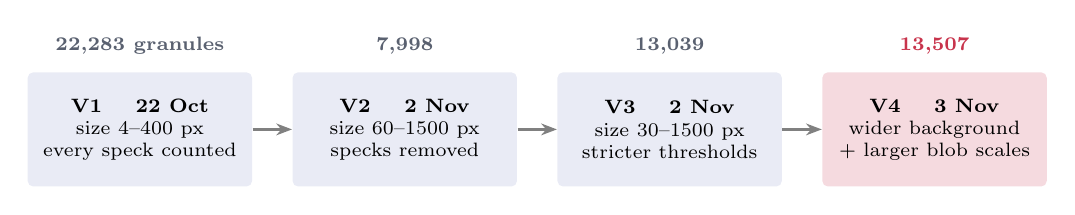
\begin{tikzpicture}[node distance=5mm,
      st/.style={fill=box,rounded corners=2pt,minimum width=2.85cm,minimum height=1.45cm,align=center,font=\scriptsize},
      ar/.style={-{Stealth[length=2mm]},thick,gray}]
    \node[st] (a) {\textbf{V1 \quad 22 Oct}\\ size 4--400 px\\ every speck counted};
    \node[st,right=of a] (b) {\textbf{V2 \quad 2 Nov}\\ size 60--1500 px\\ specks removed};
    \node[st,right=of b] (c) {\textbf{V3 \quad 2 Nov}\\ size 30--1500 px\\ stricter thresholds};
    \node[st,right=of c,fill=big!18] (d) {\textbf{V4 \quad 3 Nov}\\ wider background\\ + larger blob scales};
    \draw[ar] (a) -- (b); \draw[ar] (b) -- (c); \draw[ar] (c) -- (d);
    \node[font=\scriptsize\bfseries,color=muted,above=1mm of a] {22,283 granules};
    \node[font=\scriptsize\bfseries,color=muted,above=1mm of b] {7,998};
    \node[font=\scriptsize\bfseries,color=muted,above=1mm of c] {13,039};
    \node[font=\scriptsize\bfseries,color=big,above=1mm of d] {13,507};
  \end{tikzpicture}

  \vspace{5mm}
  \begin{columns}[T]
    \begin{column}{0.31\textwidth}\bignum{0.34 $\rightarrow$ 0.52}{UNet F1 on the hand labels}\end{column}
    \begin{column}{0.31\textwidth}\bignum{0.23 $\rightarrow$ 0.49}{UNet precision: false positives halved}\end{column}
    \begin{column}{0.31\textwidth}\bignum{0.73 $\rightarrow$ 0.71}{UNet recall: kept}\end{column}
  \end{columns}

  \keyidea{\textbf{Key idea:} the models learn only from these automatic labels. Each version was used to retrain the networks,
  which were then scored against the same 8 hand-labelled video-3 tiles (102 granules) that no model ever saw.}
\end{frame}

% ---------------------------------------------------------------- I.2
\begin{frame}{The same cells, labelled by each version}
  \centering
  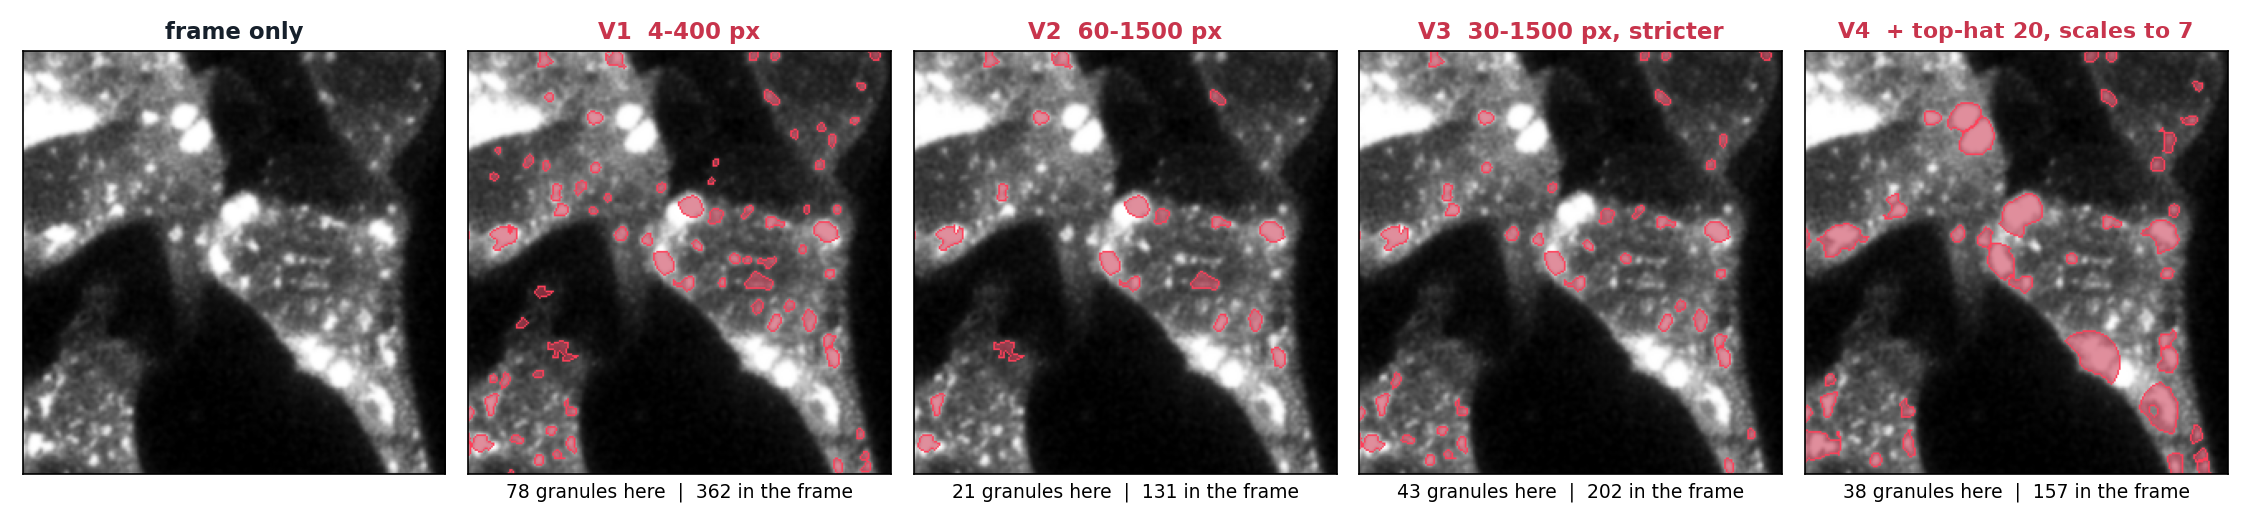
\includegraphics[width=\linewidth]{regen_versions.png}

  \vspace{2mm}
  \begin{columns}[T]
    \begin{column}{0.24\textwidth}\small\textbf{V1}: dozens of tiny specks marked as granules.\end{column}
    \begin{column}{0.24\textwidth}\small\textbf{V2}: specks gone, but real small granules too.\end{column}
    \begin{column}{0.24\textwidth}\small\textbf{V3}: small granules back, faint texture kept out.\end{column}
    \begin{column}{0.24\textwidth}\small\textbf{V4}: large bright granules outlined in full.\end{column}
  \end{columns}
  \vfill
  \src{My labelling code re-run with each version's settings on video 1, frame 10 (DATA\_FOR\_TEAM.zip). Check: the V1 re-run finds 362 granules, the stored V1 labels 366.}
\end{frame}

% ---------------------------------------------------------------- I.3
\begin{frame}{From 4--400 px to now: what each step did}
  \centering\scriptsize
  \renewcommand{\arraystretch}{1.25}\setlength{\tabcolsep}{3pt}
  \begin{tabular}{@{}p{1.35cm}p{3.9cm}ccccp{4.0cm}@{}}
    \toprule
    \textbf{Step} & \textbf{What we did} & \textbf{Prec.} & \textbf{Recall} & \textbf{F1} & \textbf{Wrong} & \textbf{In plain words} \\
    \midrule
    V1 \; 4--400 & every bright spot of 4--400 px called a granule & 0.23 & 0.73 & 0.34 & $\sim$250
      & finds most granules, but 3 of every 4 marks are wrong \\
    V2 \; 60--1500 & dropped every blob under 60 px (professor: too many false positives)
      & 0.48 & 0.38 & 0.37 & 41 & false marks almost gone, but now 6 of 10 real granules are missed \\
    V3 \; 30--1500 & minimum back to 30 px, stricter brightness test ($k$ 4 $\rightarrow$ 5, contrast 0.5 $\rightarrow$ 0.7)
      & 0.43 & 0.65 & 0.46 & 88 & the small real granules come back; faint texture stays out \\
    V4 \; final & top-hat radius 8 $\rightarrow$ 20 px; blob scales up to $\sigma$ = 7
      & 0.49 & 0.71 & 0.52 & 75 & big granules outlined in full: dice 0.55 $\rightarrow$ 0.70 \\
    \rowcolor{box}\textbf{+ filter} & after prediction, delete blobs under 20 px; \textbf{no retraining}
      & \textbf{0.56} & \textbf{0.71} & \textbf{0.57} & \textbf{56} & a quarter of the false marks go, no real granule lost \\
    \bottomrule
  \end{tabular}

  \vspace{3mm}
  \begin{columns}[T]
    \begin{column}{0.31\textwidth}\bignum{2.4$\times$}{precision 0.23 $\rightarrow$ 0.56; recall kept at 0.71}\end{column}
    \begin{column}{0.31\textwidth}\bignum{$\sim$250 $\rightarrow$ 56}{wrong detections on the 8 hand tiles}\end{column}
    \begin{column}{0.31\textwidth}\bignum{0.38 $\rightarrow$ 0.53}{labeller F1 (V1 on 8 tiles, V4 on 7)}\end{column}
  \end{columns}
  \src{UNet on the 8 hand-labelled video-3 tiles (102 granules), mean of 5 checkpoints. Wrong = false positives. V1: Phase-1 deck (its count worked out from precision and recall); V2--V4: Rahul's v3\_tiles\_extra.csv; filter: blob\_filter\_results. All tables: group7\_results\_journey.xlsx.}
\end{frame}

% ---------------------------------------------------------------- I.4
\begin{frame}{V4 keeps V1's recall at twice the precision}
  \centering
  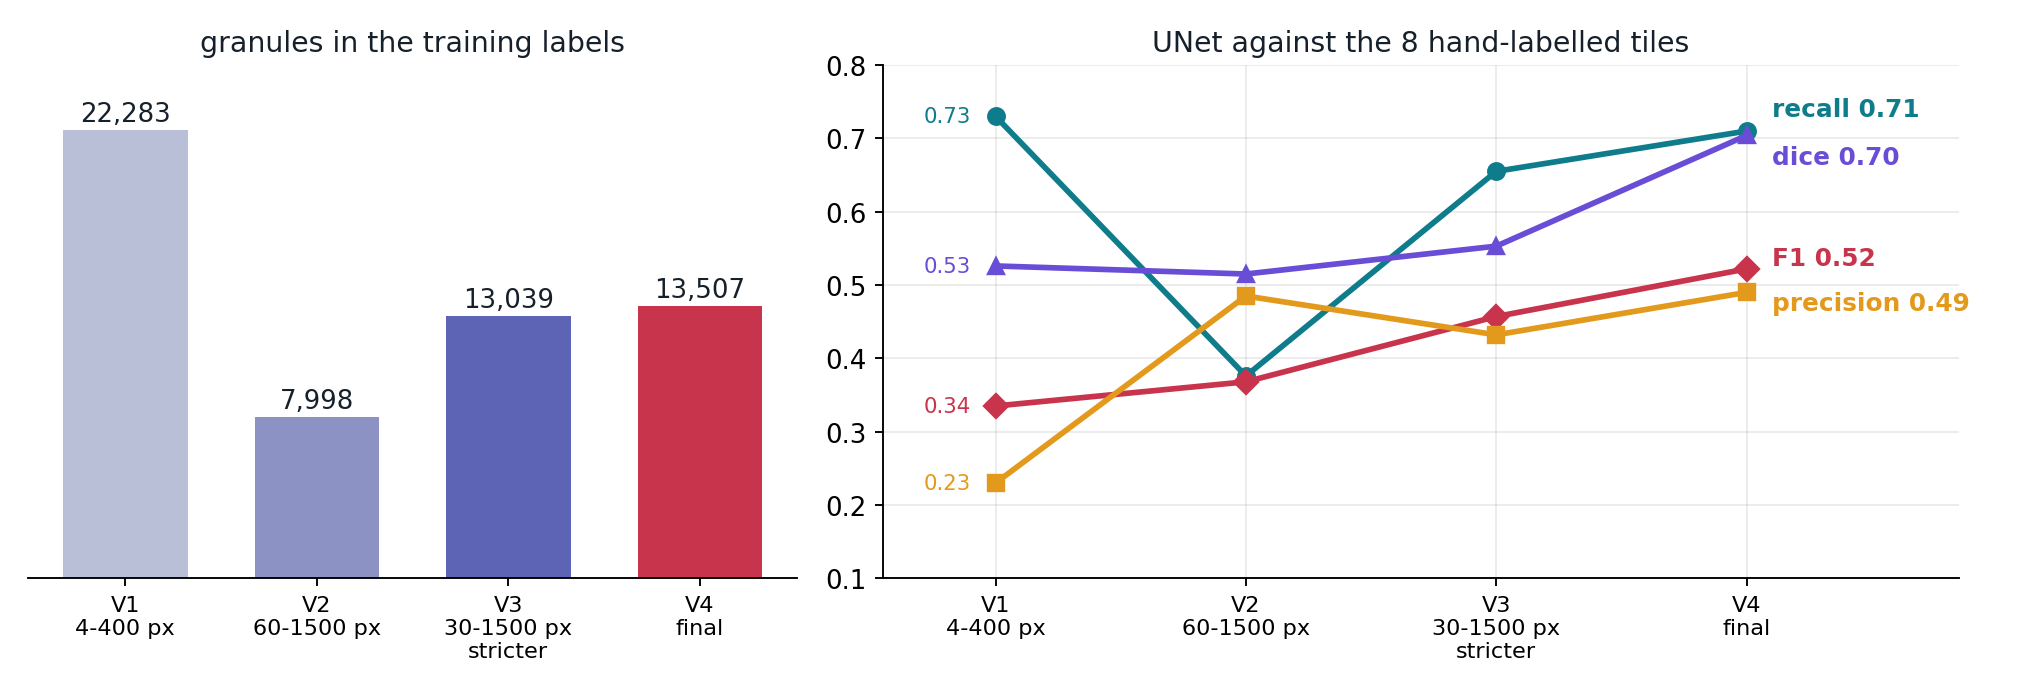
\includegraphics[width=\linewidth]{evolution.png}

  \vspace{1mm}
  \begin{columns}[T]
    \begin{column}{0.48\textwidth}\small
      Fewer granules in the labels (V2) cut false positives but lost recall. V3 and V4 recovered it without the specks.
    \end{column}
    \begin{column}{0.48\textwidth}\small
      Every network gained: F1 from V2 to V4 rose by 0.12--0.19 for NoSkip, UNet, AttUNet, DWUNet and DWAttUNet.
    \end{column}
  \end{columns}
  \src{Granules: videos 1+2, all tiles (tp + fn of Rahul's 5-fold runs). UNet scores: counts summed over the 8 tiles, mean of the checkpoints.}
\end{frame}

% ---------------------------------------------------------------- I.5
\begin{frame}{Large granules are found; tiny blobs cause the false positives}
  \centering
  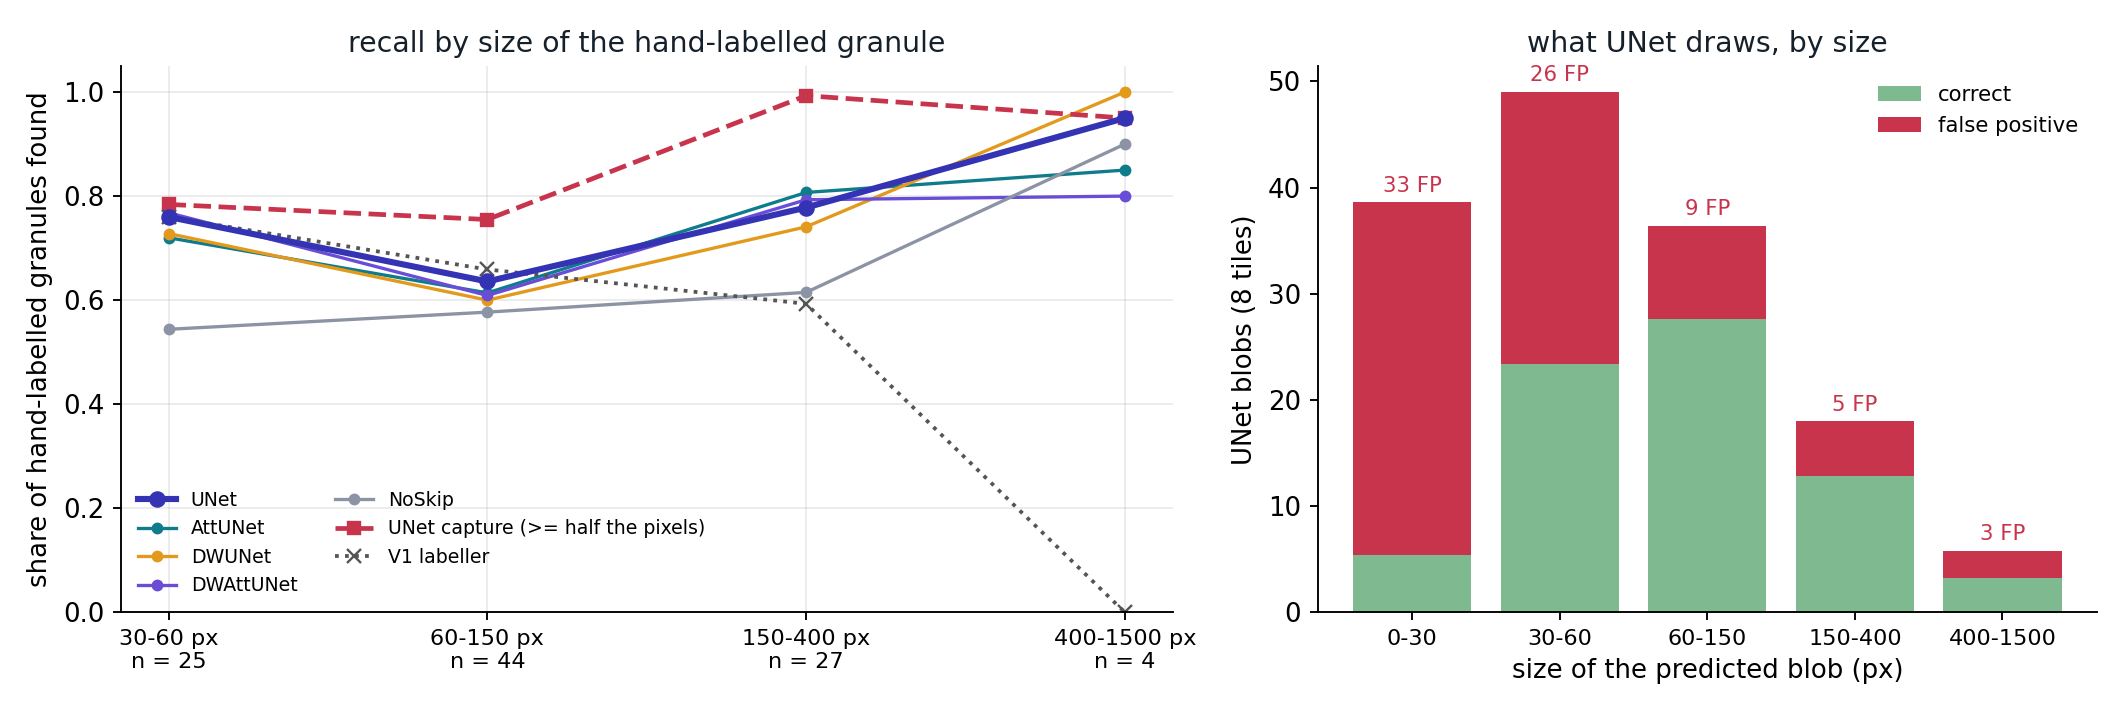
\includegraphics[width=\linewidth]{size_scores.png}

  \vspace{1mm}
  \begin{columns}[T]
    \begin{column}{0.31\textwidth}\bignum{0.80 \,/\, 99\%}{UNet recall / capture for granules $\geq$ 150 px (31 hand granules); 0.68 / 77\% for 30--150 px}\end{column}
    \begin{column}{0.31\textwidth}\bignum{44\%}{of UNet's false positives are blobs under 30 px, a size the labels never contain}\end{column}
    \begin{column}{0.31\textwidth}\bignum{0.49 $\rightarrow$ 0.56}{UNet precision after dropping predicted blobs under 20 px, no retraining; recall stays 0.71, F1 0.52 $\rightarrow$ 0.57. Every network gains}\end{column}
  \end{columns}
  \src{Hand labels, 8 tiles, mean of 5 checkpoints; capture = at least half of the granule predicted. Blob filter: 20 px chosen on validation tiles only; 5-fold test precision 0.64 $\rightarrow$ 0.72, F1 0.66 $\rightarrow$ 0.70.
  Against the pseudo-labels (5 folds), large granules: recall 0.64, about a fifth merged. The V1 labeller found 0 of the 4 granules over 400 px.}
\end{frame}

% ---------------------------------------------------------------- I.6
\begin{frame}{Perimeters, and how granule size changes over time}
  \centering
  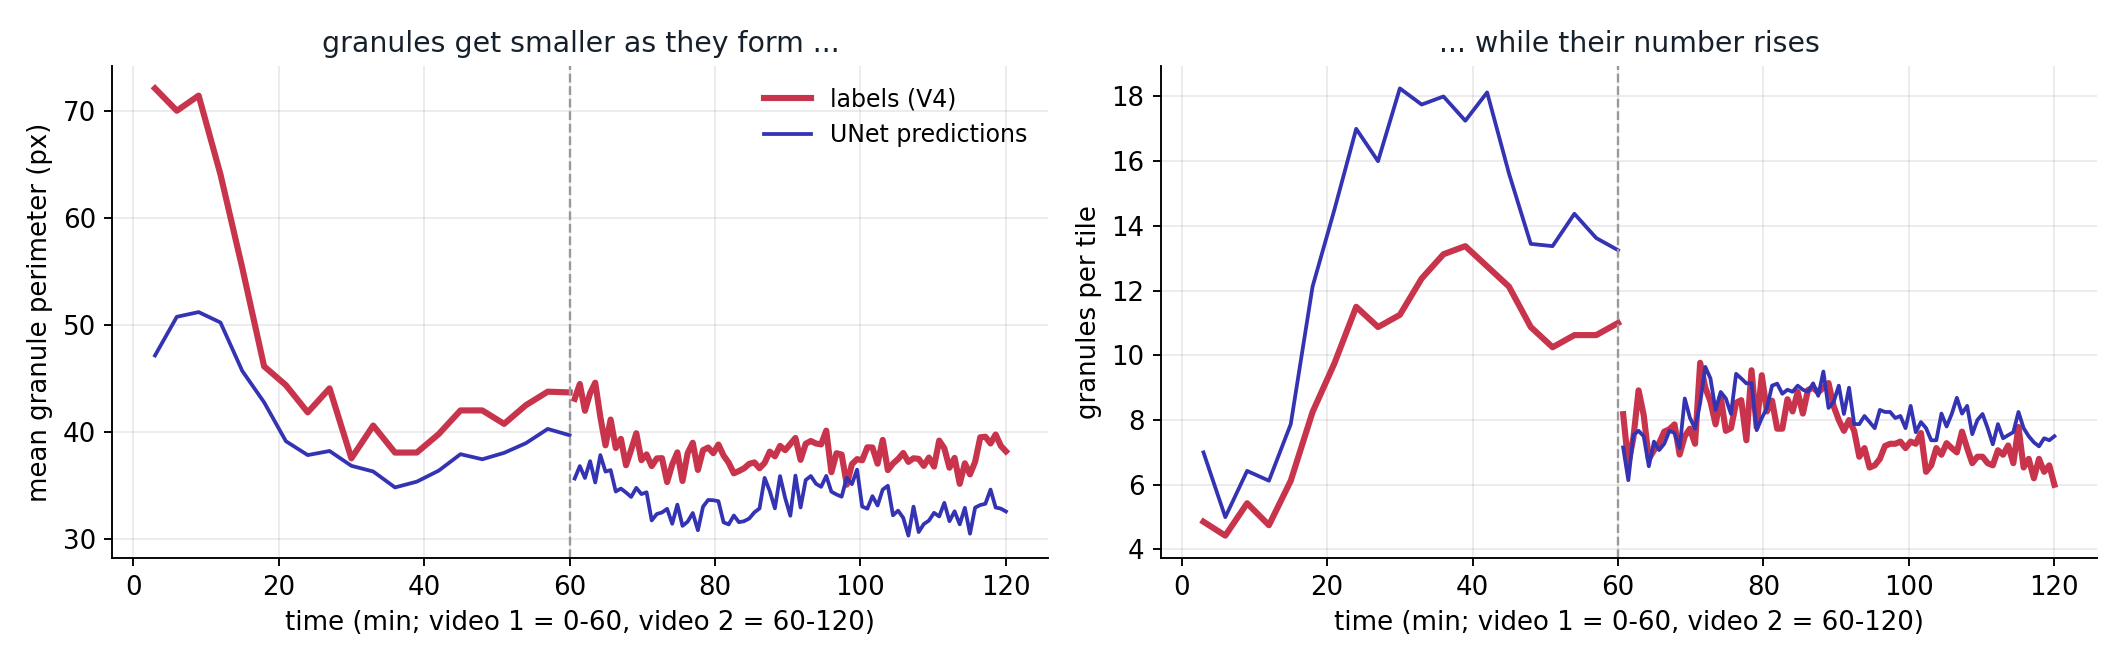
\includegraphics[height=3.75cm,keepaspectratio]{size_time.png}

  \vspace{1mm}
  \begin{columns}[c]
    \begin{column}{0.45\textwidth}
      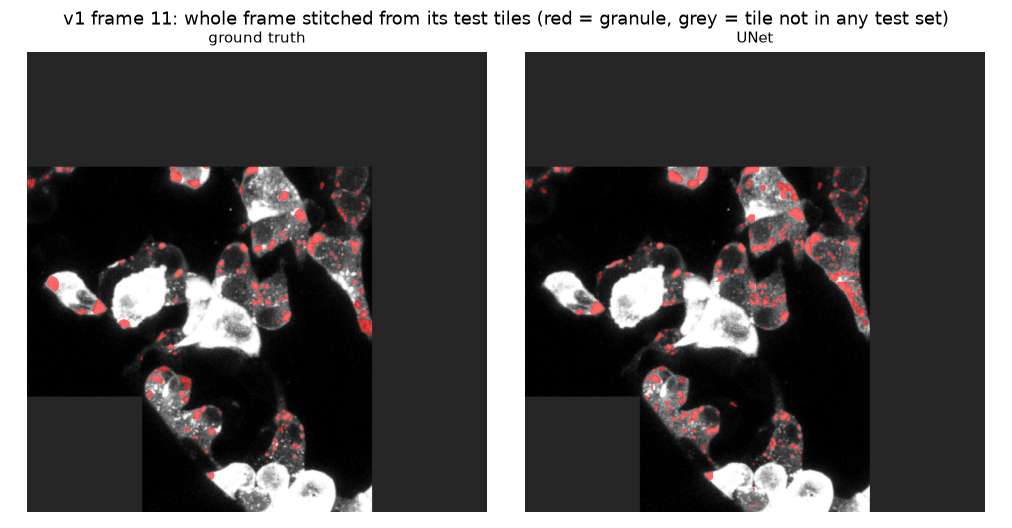
\includegraphics[width=\linewidth]{heatmap_red_frame_v1.png}
    \end{column}
    \begin{column}{0.52\textwidth}\small
      \textbf{\color{big}Perimeter}: hand-labelled granules have a median of 35 px; 64\% lie between 20 and 45 px.
      UNet outlines are within 7\% of the labeller's, but 14\% shorter than hand-drawn ones.\par\vspace{1.5mm}
      \textbf{\color{big}Time}: in video 1 the granules per tile rise from about 5 to 13 while the mean perimeter falls from about 70 to 40 px
      ($p < 0.001$): many small new granules appear. UNet follows the same trend, though it over-counts.
    \end{column}
  \end{columns}
  \src{5-fold test sets: every video-1/2 tile is predicted once, by the fold that held it out. Time from the video names (0--60, 60--120 min). Left: video 1, frame 11, red = granule.}
\end{frame}

% ================================================================ PART II  (Rahul)
\partslide{Part II \textperiodcentered\ Architecture ablation}{From FCN to Attention U-Net: what actually helps?}
  {Five encoder-decoder networks across 5 folds, evaluated on held-out pseudo-labels and 8 unseen hand-labelled tiles}
  {Rahul Joseph Bejoy \quad{\normalfont\small\ttfamily CH24BTECH11031 \textperiodcentered\ Ablation study \& post-processing}}

% ---------------------------------------------------------------- II.1
\begin{frame}{Five networks test skip connections, attention and filter efficiency}
  \centering\footnotesize
  \renewcommand{\arraystretch}{1.3}\setlength{\tabcolsep}{4pt}
  \begin{tabular}{@{}lp{3.2cm}rccp{3.5cm}@{}}
    \toprule
    \textbf{Model} & \textbf{Architecture} & \textbf{Parameters} & \textbf{Size} & \textbf{Train (min)} & \textbf{What it tests} \\
    \midrule
    NoSkip & encoder-decoder without skips & 1,747,921 & 0.90$\times$ & 10.9 & FCN baseline without spatial skip paths \\
    \hl\textbf{\color{big}UNet} & \textbf{\color{big}NoSkip + encoder-decoder skips} & \textbf{\color{big}1,943,761} & \textbf{\color{big}1.00$\times$} & \textbf{\color{big}10.0}
      & \textbf{\color{big}fine-detail recovery via skip connections} \\
    AttUNet & UNet + soft attention gates & 1,965,885 & 1.01$\times$ & 12.7 & gating skip features before concatenation \\
    DWUNet & UNet with depthwise-separable convolutions & 389,435 & 0.20$\times$ & 14.3 & 5$\times$ lighter: parameter efficiency \\
    DWAttUNet & depthwise-separable + attention & 411,559 & 0.21$\times$ & 14.6 & combined lightweight + attention \\
    \bottomrule
  \end{tabular}

  \vspace{5mm}
  \begin{columns}[T]
    \begin{column}{0.31\textwidth}\bignum{5$\times$ fewer}{parameters in DWUNet (389k vs 1.94M)}\end{column}
    \begin{column}{0.31\textwidth}\bignum{Base width 16}{ReLU + BatchNorm + 1$\times$1 conv + sigmoid}\end{column}
    \begin{column}{0.31\textwidth}\bignum{25 checkpoints}{5 models $\times$ 5 grouped folds, on an M3 GPU}\end{column}
  \end{columns}
\end{frame}

% ---------------------------------------------------------------- II.2
\begin{frame}{Skip connections speed up convergence and lower the training loss}
  \centering
  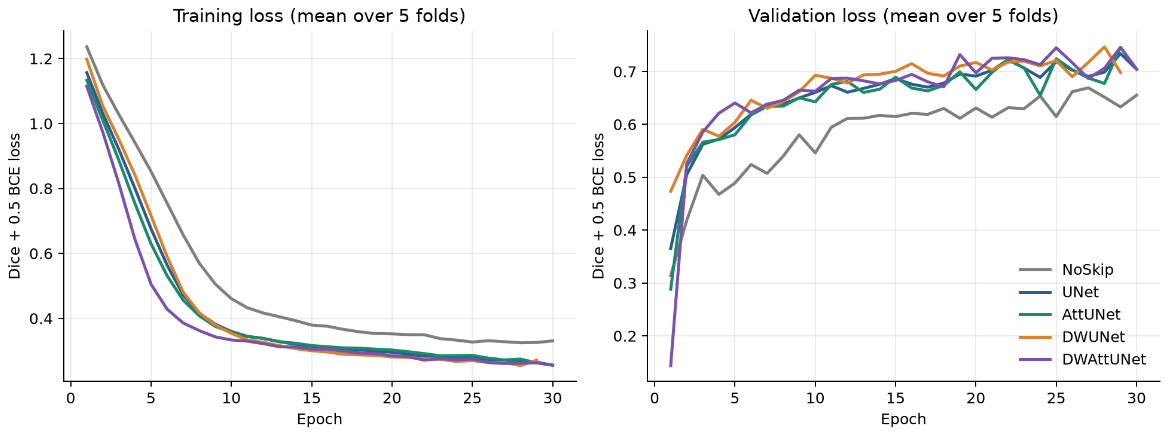
\includegraphics[height=4.6cm,keepaspectratio]{rv_loss.png}

  \vspace{2mm}
  \begin{columns}[T]
    \begin{column}{0.31\textwidth}\small\textbf{Grouped 5-fold split:} 256$\times$256 px tiles grouped by grid position; the last 15\% of frames held out for early stopping.\end{column}
    \begin{column}{0.31\textwidth}\small\textbf{Loss \& optimiser:} Dice + 0.5$\times$BCE, Adam (lr $10^{-3}$, batch 16), patience 6, at most 30 epochs.\end{column}
    \begin{column}{0.31\textwidth}\small\textbf{Augmentation:} random flips, 90$^\circ$ rotations, brightness/contrast jitter; output thresholded at 0.5.\end{column}
  \end{columns}
\end{frame}

% ---------------------------------------------------------------- II.3
\begin{frame}{Validation chooses a 20 px minimum blob size, without retraining}
  \centering
  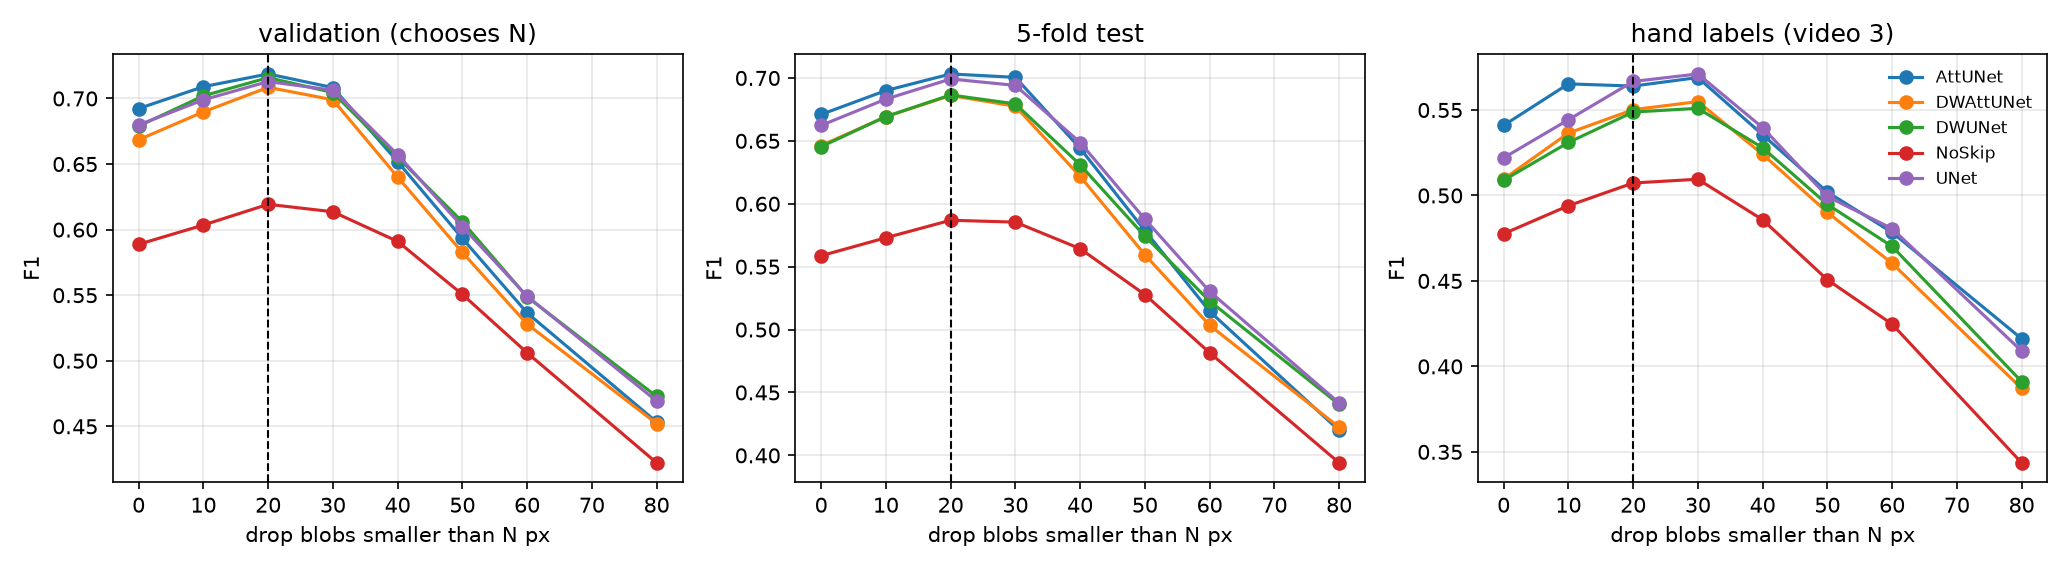
\includegraphics[width=\linewidth]{rv_sweep.png}

  \vspace{2mm}
  \begin{columns}[T]
    \begin{column}{0.31\textwidth}\bignum{N = 20 px}{chosen on validation tiles only (mean F1 0.662 $\rightarrow$ 0.695)}\end{column}
    \begin{column}{0.31\textwidth}\bignum{\color{blu}0.64 $\rightarrow$ 0.72}{UNet 5-fold test precision (F1 +0.037)}\end{column}
    \begin{column}{0.31\textwidth}\bignum{\color{grn}75.4 $\rightarrow$ 55.8}{UNet false positives on the hand tiles (F1 0.522 $\rightarrow$ 0.567)}\end{column}
  \end{columns}
  \src{Predicted blobs smaller than N px are deleted after the 0.5 threshold. Dashed line: the chosen N.}
\end{frame}

% ---------------------------------------------------------------- II.4
\begin{frame}{Skip connections add +0.11 F1; attention and depthwise match the standard UNet}
  \centering\scriptsize
  \renewcommand{\arraystretch}{1.35}\setlength{\tabcolsep}{4pt}
  \begin{tabular}{@{}lcccccc@{}}
    \toprule
    \textbf{Model} & \textbf{5-fold F1} & \textbf{5-fold F1} & \textbf{5-fold IoU} & \textbf{Hand prec. / rec.} & \textbf{Hand F1} & \textbf{Hand FP} \\
     & (N = 0) & (N = 20) & (N = 20) & (N = 20) & (N = 0 $\rightarrow$ 20) & (N = 0 $\rightarrow$ 20) \\
    \midrule
    NoSkip & 0.559 $\pm$ 0.044 & 0.587 $\pm$ 0.043 & 0.716 $\pm$ 0.020 & 0.509 / 0.578 & 0.478 $\rightarrow$ 0.507 & 69.4 $\rightarrow$ 57.0 \\
    \hl\textbf{\color{big}UNet} & \textbf{\color{big}0.662 $\pm$ 0.045} & \textbf{\color{big}0.699 $\pm$ 0.039} & \textbf{\color{big}0.824 $\pm$ 0.011}
      & \textbf{\color{big}0.563 / 0.706} & \textbf{\color{big}0.522 $\rightarrow$ 0.567} & \textbf{\color{big}75.4 $\rightarrow$ 55.8} \\
    \hl\textbf{\color{big}AttUNet} & \textbf{\color{big}0.671 $\pm$ 0.050} & \textbf{\color{big}0.703 $\pm$ 0.047} & \textbf{\color{big}0.827 $\pm$ 0.024}
      & \textbf{\color{big}0.568 / 0.690} & \textbf{\color{big}0.541 $\rightarrow$ 0.564} & \textbf{\color{big}69.2 $\rightarrow$ 53.6} \\
    DWUNet & 0.645 $\pm$ 0.049 & 0.686 $\pm$ 0.045 & 0.833 $\pm$ 0.015 & 0.550 / 0.669 & 0.509 $\rightarrow$ 0.549 & 74.8 $\rightarrow$ 55.8 \\
    DWAttUNet & 0.646 $\pm$ 0.044 & 0.686 $\pm$ 0.048 & 0.820 $\pm$ 0.018 & 0.543 / 0.692 & 0.510 $\rightarrow$ 0.550 & 82.0 $\rightarrow$ 59.4 \\
    \bottomrule
  \end{tabular}

  \vfill
  \keyidea{\textbf{Key takeaway:} removing the skip connections (NoSkip) causes a severe drop in IoU (0.716 vs 0.824) and recall
  (0.578 vs 0.706 on the hand labels). Adding attention gates or 5$\times$ lighter depthwise convolutions gives virtually identical accuracy.}
\end{frame}

% ---------------------------------------------------------------- II.5
\begin{frame}{Side by side on unseen hand-labelled tiles (green = TP, red = FP, yellow = FN)}
  \centering
  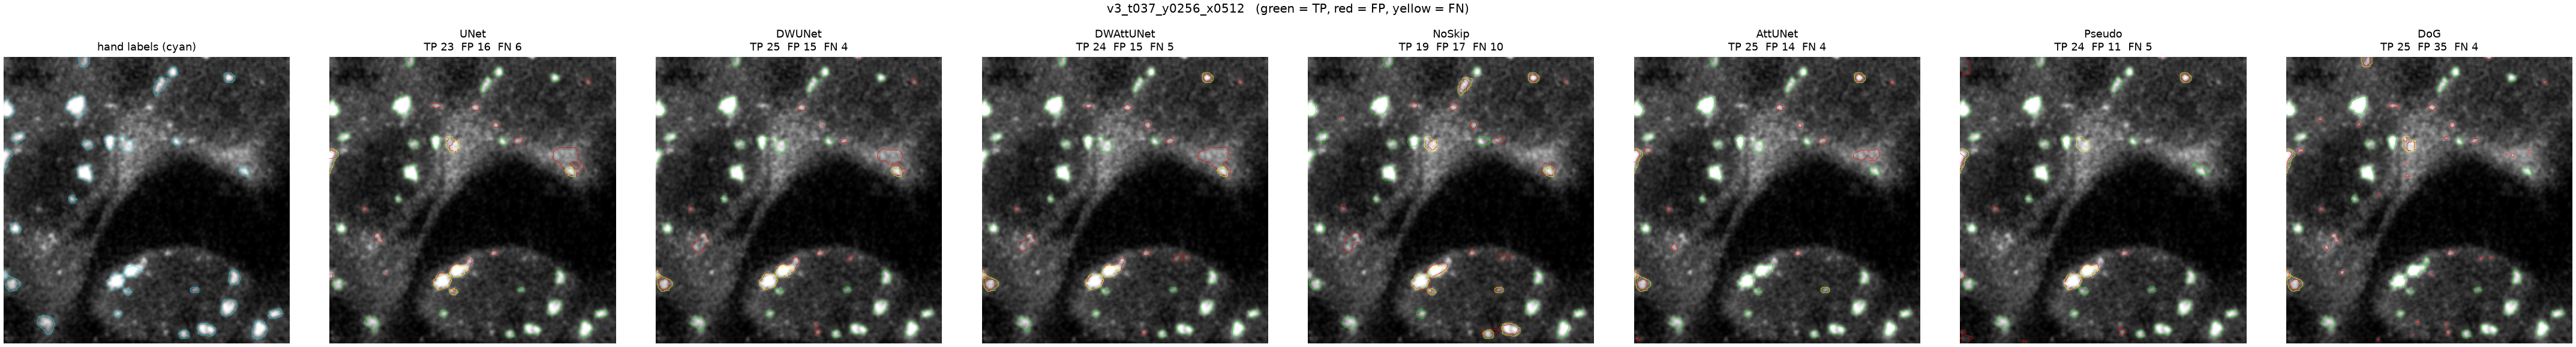
\includegraphics[width=\linewidth]{rv_overlay_a.png}\par\vspace{2mm}
  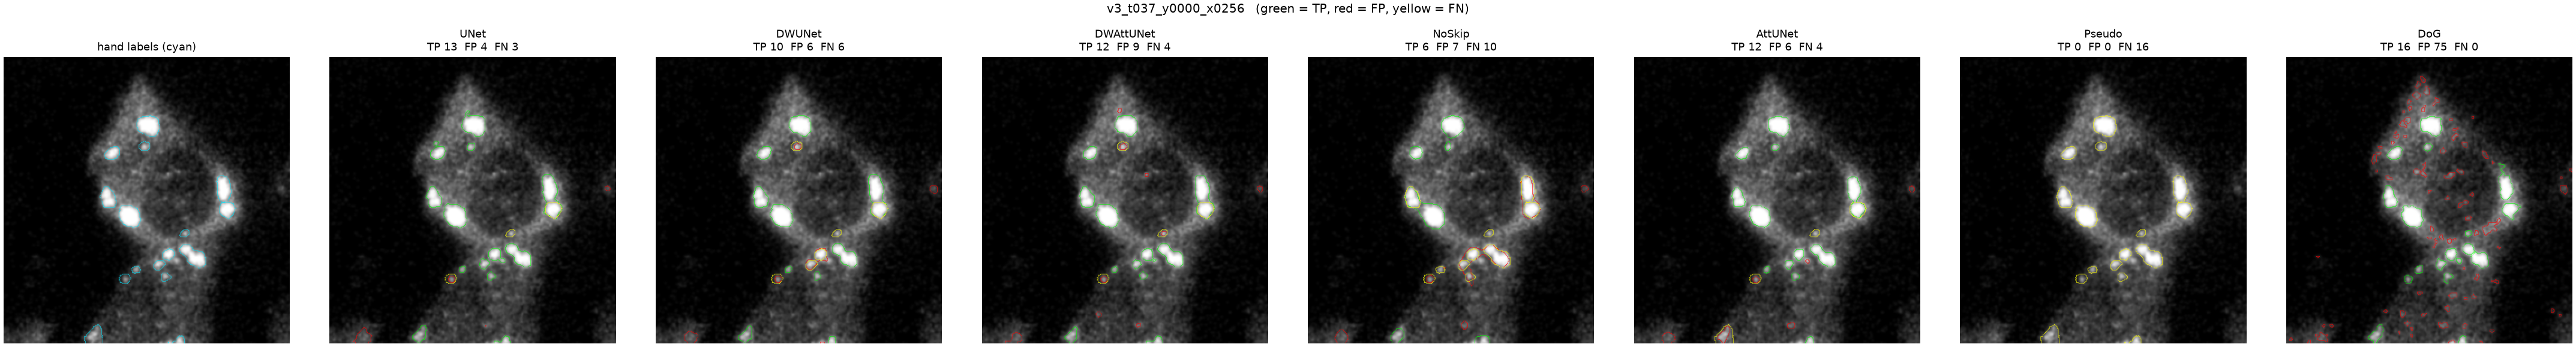
\includegraphics[width=\linewidth]{rv_overlay_b.png}

  \vfill
  \keyidea{\textbf{Visual insight:} NoSkip misses small granules (10 missed in each tile). UNet recovers them: on tile t037\_y0000\_x0256
  it finds 13 of the 16 granules (AttUNet 12), where the labeller has no mask (TP = 0).}
  \src{Panels: hand labels, UNet, DWUNet, DWAttUNet, NoSkip, AttUNet, labeller, DoG. Fold-1 checkpoints, before the blob filter.}
\end{frame}

% ================================================================ PART III  (Vedant)
\partslide{Part III \textperiodcentered\ Statistical testing \& classical baselines}{Statistical significance, the DoG baseline, and comparison with the labeller}
  {Friedman tests, Holm-corrected paired t-tests, violin distributions, and a benchmark against classical detectors}
  {Vedant P Kumbakonam \quad{\normalfont\small\ttfamily CH24BTECH11042 \textperiodcentered\ Hypothesis testing \& classical baseline}}

% ---------------------------------------------------------------- III.1
\begin{frame}{Skip-connected networks form a tight cluster well above NoSkip across all 5 folds}
  \centering
  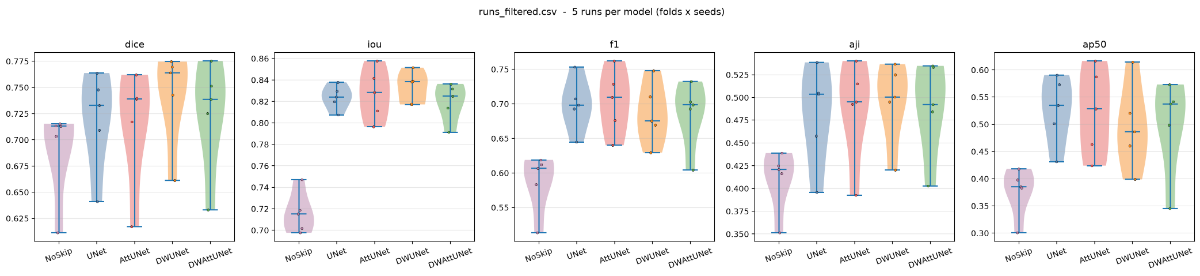
\includegraphics[width=\linewidth]{rv_violins_folds.png}

  \vspace{3mm}
  \begin{columns}[T]
    \begin{column}{0.31\textwidth}\card{Friedman test significant}{Significant model differences on F1 ($p$ = 0.007) and IoU ($p$ = 0.011).}\end{column}
    \begin{column}{0.31\textwidth}\card{NoSkip clearly inferior}{The entire IoU and F1 violin of NoSkip sits below all four U-Net variants.}\end{column}
    \begin{column}{0.31\textwidth}\card{Why a paired t-test?}{With 5 folds, Wilcoxon's smallest possible $p$-value is 0.0625, so paired t-tests + Holm are used.}\end{column}
  \end{columns}
  \src{5-fold test sets with the 20 px blob filter (runs\_filtered.csv), one point per fold.}
\end{frame}

% ---------------------------------------------------------------- III.2
\begin{frame}{All 4 U-Net variants beat NoSkip ($p_{\mathrm{holm}} < 0.01$); no difference among the 4}
  \centering\scriptsize
  \renewcommand{\arraystretch}{1.35}\setlength{\tabcolsep}{4pt}
  \begin{tabular}{@{}lcccccc@{}}
    \toprule
    \textbf{Pair (A vs B)} & \textbf{F1 diff (A $-$ B)} & \textbf{F1 $p_{\mathrm{holm}}$} & \textbf{IoU diff} & \textbf{IoU $p_{\mathrm{holm}}$} & \textbf{AJI $p_{\mathrm{holm}}$} & \textbf{Cohen's $d_z$ (F1)} \\
    \midrule
    \hl\textbf{\color{big}UNet vs NoSkip} & \textbf{\color{big}+0.112} & \textbf{\color{big}0.0040 (sig.)} & \textbf{\color{big}+0.108} & \textbf{\color{big}0.0021 (sig.)} & \textbf{\color{big}0.0340 (sig.)} & \textbf{\color{big}4.61} \\
    \hl\textbf{\color{big}AttUNet vs NoSkip} & \textbf{\color{big}+0.116} & \textbf{\color{big}0.0022 (sig.)} & \textbf{\color{big}+0.111} & \textbf{\color{big}0.0013 (sig.)} & \textbf{\color{big}0.0250 (sig.)} & \textbf{\color{big}5.54} \\
    \hl\textbf{\color{big}DWUNet vs NoSkip} & \textbf{\color{big}+0.100} & \textbf{\color{big}0.0086 (sig.)} & \textbf{\color{big}+0.117} & \textbf{\color{big}0.0008 (sig.)} & \textbf{\color{big}0.0121 (sig.)} & \textbf{\color{big}3.65} \\
    \hl\textbf{\color{big}DWAttUNet vs NoSkip} & \textbf{\color{big}+0.099} & \textbf{\color{big}0.0012 (sig.)} & \textbf{\color{big}+0.103} & \textbf{\color{big}0.0006 (sig.)} & \textbf{\color{big}0.0250 (sig.)} & \textbf{\color{big}6.67} \\
    UNet vs AttUNet & $-$0.004 & 1.000 (n.s.) & $-$0.003 & 1.000 (n.s.) & 1.000 (n.s.) & $-$0.16 \\
    UNet vs DWUNet & +0.013 & 0.874 (n.s.) & $-$0.009 & 0.521 (n.s.) & 1.000 (n.s.) & 0.63 \\
    \bottomrule
  \end{tabular}

  \vfill
  \keyidea{\textbf{Statistical conclusion:} skip connections are statistically indispensable on every metric (IoU, F1, AJI, AP50).
  Between UNet, AttUNet, DWUNet and DWAttUNet all Holm-adjusted $p$-values are 0.37--1.00: no provable difference.}
  \src{Paired t-tests on the 5 per-fold means, Holm correction over the 10 pairs of each metric. 5-fold test sets, 20 px blob filter.}
\end{frame}

% ---------------------------------------------------------------- III.3
\begin{frame}{On the 8 hand-labelled tiles, tile-to-tile variance dominates ($p_{\mathrm{holm}}$ = 1.00)}
  \centering
  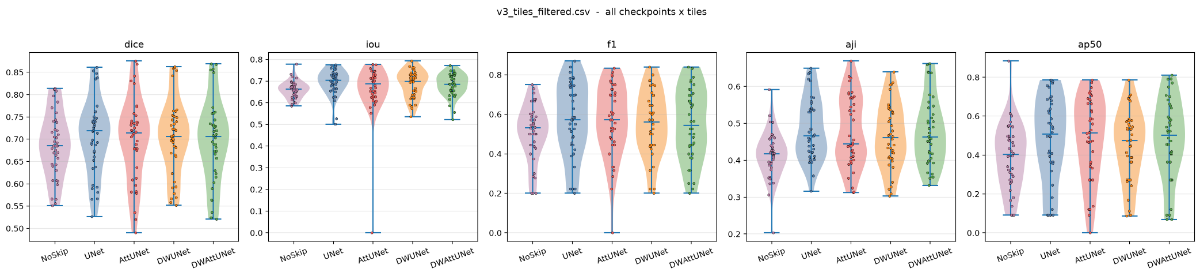
\includegraphics[width=\linewidth]{rv_violins_hand.png}

  \vspace{3mm}
  \begin{columns}[T]
    \begin{column}{0.31\textwidth}\bignum{\color{blu}0.567 vs 0.507}{UNet vs NoSkip mean F1 on the 8 unseen hand tiles}\end{column}
    \begin{column}{0.31\textwidth}\bignum{8 paired tiles}{low statistical power across tiles: treat rankings as indicative}\end{column}
    \begin{column}{0.31\textwidth}\bignum{\color{grn}0.705 dice}{UNet has the highest pixel overlap with the human outlines}\end{column}
  \end{columns}
  \src{All checkpoints $\times$ tiles, 20 px blob filter (v3\_tiles\_filtered.csv).}
\end{frame}

% ---------------------------------------------------------------- III.4
\begin{frame}{DoG over-detects (714 FPs); trained networks match the V4 labeller}
  \centering\scriptsize
  \renewcommand{\arraystretch}{1.3}
  \begin{tabular}{@{}lccccrrr@{}}
    \toprule
    \textbf{Method (8 hand tiles, 102 granules)} & \textbf{F1} & \textbf{Precision} & \textbf{Recall} & \textbf{Dice} & \textbf{TP (found)} & \textbf{FP (wrong)} & \textbf{FN (missed)} \\
    \midrule
    \hl\textbf{\color{big}UNet (N = 20 filter)} & \textbf{\color{big}0.567} & \textbf{\color{big}0.563} & \textbf{\color{big}0.706} & \textbf{\color{big}0.705} & \textbf{\color{big}72.0} & \textbf{\color{big}55.8} & \textbf{\color{big}30.0} \\
    \hl\textbf{\color{big}AttUNet (N = 20 filter)} & \textbf{\color{big}0.564} & \textbf{\color{big}0.568} & \textbf{\color{big}0.690} & \textbf{\color{big}0.697} & \textbf{\color{big}70.4} & \textbf{\color{big}53.6} & \textbf{\color{big}31.6} \\
    DWAttUNet (N = 20 filter) & 0.550 & 0.543 & 0.692 & 0.694 & 70.6 & 59.4 & 31.4 \\
    DWUNet (N = 20 filter) & 0.549 & 0.550 & 0.669 & 0.704 & 68.2 & 55.8 & 33.8 \\
    NoSkip (N = 20 filter) & 0.507 & 0.509 & 0.578 & 0.688 & 59.0 & 57.0 & 43.0 \\
    V4 labeller (7 tiles) & 0.533 & 0.579 & 0.640 & 0.651 & 55.0 & 40.0 & 31.0 \\
    DoG (classical baseline) & 0.224 & 0.102 & 0.794 & 0.502 & 81.0 & 714.0 & 21.0 \\
    \bottomrule
  \end{tabular}

  \vfill
  \keyidea{\textbf{Baseline verdict:} the classical Difference of Gaussians (DoG) catches 79\% of the granules but floods the tiles with
  714 false positives (F1 0.224). With the 20 px filter, UNet and AttUNet reach F1 $\approx$ 0.567 and a higher dice than the labeller they learned from (0.705 vs 0.651).}
  \src{The labeller mask of one tile is missing, so it is scored on 7 tiles. On those same 7 tiles (no filter) UNet still has the higher dice: 0.68 vs 0.65.}
\end{frame}

% ================================================================ CLOSING
\begin{frame}{Better labels and blob splitting matter more than heavier architectures}
  \vspace{4mm}
  \begin{columns}[T]
    \begin{column}{0.31\textwidth}\card{Pseudo-label ceiling}{Student networks cannot vastly exceed their teacher's masks; fine-tuning on a few human-labelled tiles is next.}\end{column}
    \begin{column}{0.31\textwidth}\card{Touching granules merge}{Connected-component masks merge adjacent blobs (16--24\% of granules over 60 px); watershed splitting should raise AJI.}\end{column}
    \begin{column}{0.31\textwidth}\card{Lightweight deployment}{DWUNet matches UNet with 5$\times$ fewer parameters: well suited to fast bio-image deployment.}\end{column}
  \end{columns}

  \vspace{6mm}
  \keyidea{\textbf{Where the gains came from:} better labels (F1 0.34 $\rightarrow$ 0.52) and a 20 px post-filter (0.52 $\rightarrow$ 0.57)
  improved every network; changing the architecture beyond adding skip connections did not.}
  \src{Merge rate: UNet on the 5-fold test sets, granules of 60--150, 150--400 and 400--1500 px (backup slide B7).}
\end{frame}

% ---------------------------------------------------------------- backup: every table (generated, see backup.tex)
\appendix
\begin{frame}{Backup slides: all the tables}
  \centering\small
  \begin{tabular}{@{}rl@{}}
    B1 & Every network, every step, on the hand tiles \\
    B2 & The labeller settings of each version, and what each setting means \\
    B3 & The labeller, DoG and the networks on the hand tiles \\
    B4 & 5-fold cross-validation for every version \\
    B5 & The blob filter, every minimum size \\
    B6 & Scores by granule size and perimeter: hand tiles \\
    B7 & Scores by granule size and perimeter: 5-fold test sets \\
    B8 & Perimeter ranges and change over time \\
    B9 & The words used in these tables \\
    B10 & Heatmap: where granules form, labels vs every network \\
    B11--B12 & Heatmaps: all 8 hand-labelled tiles, every method \\
    B13 & Heatmap: a whole video-2 frame, labels vs UNet \\
    B14 & Heatmaps: 5-fold test tiles, labels vs UNet \\
  \end{tabular}
  \vfill
  \src{The same numbers are in group7\_results\_journey.xlsx.}
\end{frame}

% Backup slides, generated from the same data as group7_results_journey.xlsx
\begin{frame}{Backup: every network, every step (hand-labelled tiles)}
  \centering\scriptsize
  \renewcommand{\arraystretch}{1.05}\setlength{\tabcolsep}{3.5pt}
  Precision / recall / \textbf{F1}\\[1mm]
\begin{tabular}{@{}lccccc@{}}
\toprule
\textbf{Model} & \textbf{V1 4--400} & \textbf{V2 60--1500} & \textbf{V3 30--1500} & \textbf{V4 final} & \textbf{+ filter} \\
\midrule
NoSkip & -- & 0.47 / 0.32 / \textbf{0.36} & 0.39 / 0.54 / \textbf{0.39} & 0.46 / 0.58 / \textbf{0.48} & 0.51 / 0.58 / \textbf{0.51} \\
UNet & 0.23 / 0.73 / \textbf{0.34} & 0.48 / 0.38 / \textbf{0.37} & 0.43 / 0.65 / \textbf{0.46} & 0.49 / 0.71 / \textbf{0.52} & 0.56 / 0.71 / \textbf{0.57} \\
AttUNet & -- & 0.42 / 0.39 / \textbf{0.35} & 0.44 / 0.67 / \textbf{0.46} & 0.51 / 0.70 / \textbf{0.54} & 0.57 / 0.69 / \textbf{0.56} \\
DWUNet & 0.21 / 0.72 / \textbf{0.30} & 0.45 / 0.37 / \textbf{0.35} & 0.40 / 0.63 / \textbf{0.42} & 0.48 / 0.67 / \textbf{0.51} & 0.55 / 0.67 / \textbf{0.55} \\
DWAttUNet & 0.21 / 0.73 / \textbf{0.32} & 0.45 / 0.37 / \textbf{0.36} & 0.38 / 0.63 / \textbf{0.40} & 0.46 / 0.70 / \textbf{0.51} & 0.54 / 0.69 / \textbf{0.55} \\
\bottomrule
\end{tabular}

  \vspace{3mm}
\begin{tabular}{@{}lccccc@{}}
\toprule
\textbf{Wrong detections} & \textbf{V1 4--400} & \textbf{V2 60--1500} & \textbf{V3 30--1500} & \textbf{V4 final} & \textbf{+ filter} \\
\midrule
NoSkip & -- & 36 & 86 & 69 & 57 \\
UNet & $\sim$249 & 41 & 88 & 75 & 56 \\
AttUNet & -- & 54 & 87 & 69 & 54 \\
DWUNet & $\sim$276 & 47 & 96 & 75 & 56 \\
DWAttUNet & $\sim$280 & 45 & 104 & 82 & 59 \\
\bottomrule
\end{tabular}
  \vfill
  \src{8 hand-labelled video-3 tiles (102 granules), mean of 5 checkpoints. V1 was trained only for UNet, DWUNet and DWAttUNet (Phase-1 deck; wrong detections worked out from precision and recall). Every network gains F1 0.15--0.21 from V2 to now.}
\end{frame}

\begin{frame}{Backup: the labeller settings of each version}
  \centering\scriptsize
  \renewcommand{\arraystretch}{1.05}\setlength{\tabcolsep}{3.5pt}
\begin{tabular}{@{}lccccccr@{}}
\toprule
\textbf{Version} & \textbf{Area kept (px)} & \textbf{Max radius} & \textbf{$k$} & \textbf{Min contrast} & \textbf{Top-hat (px)} & \textbf{Blob scales $\sigma$} & \textbf{Granules} \\
\midrule
V1 & 4--400 & 12 & 4 & 0.5 & 8 & 1.5, 2.5, 3.5 & 22,283 \\
V2 & 60--1500 & 22 & 4 & 0.5 & 8 & 1.5, 2.5, 3.5 & 7,998 \\
V3 & 30--1500 & 22 & 5 & 0.7 & 8 & 1.5, 2.5, 3.5 & 13,039 \\
V4 (final) & 30--1500 & 22 & 5 & 0.7 & 20 & 1.5, 2.5, 3.5, 5.0, 7.0 & 13,507 \\
\bottomrule
\end{tabular}

  \vspace{3mm}
\begin{tabular}{@{}lp{11.2cm}@{}}
\toprule
\textbf{Setting} & \textbf{What it means} \\
\midrule
\textbf{Granule area kept} & Blobs smaller or bigger than this are thrown away. \\
\textbf{Max radius} & How far a granule may grow from its centre while its outline is traced. \\
\textbf{Threshold k} & How much brighter than the noise a spot must be to count. Higher = fewer, surer granules. \\
\textbf{Min contrast ratio} & How much brighter than its surroundings a blob must be. Higher = faint texture is ignored. \\
\textbf{Top-hat radius} & Size of the window used to remove the uneven cell background. Must be wider than the biggest granule, or big granules get hollowed out. \\
\textbf{Blob scales} & The blob sizes the detector looks for. Up to 3.5 finds blobs up to about 14 px wide; up to 7 finds the big ones too. \\
\bottomrule
\end{tabular}
  \vfill
  \src{Granules: videos 1+2, all tiles. What each change did to the scores: slide 4.}
\end{frame}

\begin{frame}{Backup: the labeller, DoG and the networks on the hand tiles}
  \centering\scriptsize
  \renewcommand{\arraystretch}{1.05}\setlength{\tabcolsep}{3.5pt}
\begin{tabular}{@{}lcccccrrr@{}}
\toprule
\textbf{Method} & \textbf{Tiles} & \textbf{F1} & \textbf{Precision} & \textbf{Recall} & \textbf{Dice} & \textbf{Found} & \textbf{Wrong} & \textbf{Missed} \\
\midrule
V1 labeller & 8 & 0.38 & 0.33 & 0.64 & 0.47 & 65 & 130 & 37 \\
DoG (baseline) & 8 & 0.22 & 0.10 & 0.79 & 0.50 & 81 & 714 & 21 \\
V4 labeller & 7 & 0.53 & 0.58 & 0.64 & 0.65 & 55 & 40 & 31 \\
\bottomrule
\end{tabular}

  \vspace{3mm}
\begin{tabular}{@{}lccccr@{}}
\toprule
\textbf{Same 7 tiles} & \textbf{F1} & \textbf{Precision} & \textbf{Recall} & \textbf{Dice} & \textbf{Wrong} \\
\midrule
V4 labeller & 0.53 & 0.58 & 0.64 & 0.65 & 40 \\
NoSkip & 0.48 & 0.46 & 0.61 & 0.67 & 63.0 \\
UNet & 0.49 & 0.46 & 0.69 & 0.68 & 69.6 \\
AttUNet & 0.52 & 0.48 & 0.69 & 0.68 & 63.4 \\
DWUNet & 0.49 & 0.46 & 0.67 & 0.68 & 68.4 \\
DWAttUNet & 0.48 & 0.44 & 0.68 & 0.67 & 75.4 \\
\bottomrule
\end{tabular}
  \vfill
  \src{The V2 and V3 result files score the V1 labeller masks, so only V1 and V4 labeller rows exist. The V4 labeller mask of one tile was missing, so it is scored on 7 tiles (right: the networks on the same 7). The networks are about as good as the labeller they learned from.}
\end{frame}

\begin{frame}{Backup: 5-fold cross-validation, against each version's own labels}
  \centering\scriptsize
  \renewcommand{\arraystretch}{1.05}\setlength{\tabcolsep}{3.5pt}
\begin{tabular}{@{}lccccc@{}}
\toprule
\textbf{F1} & \textbf{V1 4--400} & \textbf{V2 60--1500} & \textbf{V3 30--1500} & \textbf{V4 final} & \textbf{+ filter} \\
\midrule
NoSkip & -- & 0.55 $\pm$ 0.04 & 0.62 $\pm$ 0.03 & 0.56 $\pm$ 0.04 & 0.59 $\pm$ 0.04 \\
UNet & 0.71 $\pm$ 0.01 & 0.62 $\pm$ 0.07 & 0.69 $\pm$ 0.03 & 0.66 $\pm$ 0.04 & 0.70 $\pm$ 0.04 \\
AttUNet & -- & 0.65 $\pm$ 0.07 & 0.71 $\pm$ 0.03 & 0.67 $\pm$ 0.05 & 0.70 $\pm$ 0.05 \\
DWUNet & 0.69 $\pm$ 0.02 & 0.61 $\pm$ 0.08 & 0.69 $\pm$ 0.03 & 0.65 $\pm$ 0.05 & 0.69 $\pm$ 0.04 \\
DWAttUNet & 0.69 $\pm$ 0.01 & 0.59 $\pm$ 0.08 & 0.67 $\pm$ 0.02 & 0.65 $\pm$ 0.04 & 0.69 $\pm$ 0.05 \\
\bottomrule
\end{tabular}

  \vspace{3mm}
\begin{tabular}{@{}lccccc@{}}
\toprule
\textbf{Precision / recall} & \textbf{V1 4--400} & \textbf{V2 60--1500} & \textbf{V3 30--1500} & \textbf{V4 final} & \textbf{+ filter} \\
\midrule
NoSkip & -- & 0.58 / 0.54 & 0.61 / 0.64 & 0.57 / 0.55 & 0.63 / 0.55 \\
UNet & 0.72 / 0.71 & 0.61 / 0.64 & 0.67 / 0.72 & 0.64 / 0.70 & 0.72 / 0.69 \\
AttUNet & -- & 0.63 / 0.68 & 0.69 / 0.74 & 0.65 / 0.70 & 0.72 / 0.69 \\
DWUNet & 0.69 / 0.69 & 0.59 / 0.64 & 0.66 / 0.71 & 0.63 / 0.66 & 0.73 / 0.65 \\
DWAttUNet & 0.69 / 0.69 & 0.57 / 0.63 & 0.63 / 0.72 & 0.62 / 0.68 & 0.70 / 0.67 \\
\bottomrule
\end{tabular}
  \vfill
  \src{Mean $\pm$ std over the 5 test folds. Each version is scored against its own automatic labels, so this shows how well the network copies the labeller --- do not read it as progress between versions (the hand tiles are the fair test). V1: 3 seeds per fold.}
\end{frame}

\begin{frame}{Backup: the blob filter, every minimum size N (UNet, and validation F1 of every network)}
  \centering\scriptsize
  \renewcommand{\arraystretch}{1.05}\setlength{\tabcolsep}{3.5pt}
\begin{tabular}{@{}lcccccccccc@{}}
\toprule
& \multicolumn{3}{c}{\textbf{Validation (chooses N)}} & \multicolumn{3}{c}{\textbf{5-fold test}} & \multicolumn{4}{c}{\textbf{Hand tiles}} \\ \cmidrule(lr){2-4}\cmidrule(lr){5-7}\cmidrule(l){8-11}
\textbf{N (px)} & \textbf{P} & \textbf{R} & \textbf{F1} & \textbf{P} & \textbf{R} & \textbf{F1} & \textbf{P} & \textbf{R} & \textbf{F1} & \textbf{Wrong} \\
\midrule
0 (as before) & 0.63 & 0.73 & 0.68 & 0.63 & 0.70 & 0.66 & 0.49 & 0.71 & 0.52 & 75 \\
10 & 0.67 & 0.73 & 0.70 & 0.67 & 0.70 & 0.68 & 0.53 & 0.71 & 0.54 & 65 \\
20 \textbf{chosen} & 0.71 & 0.72 & 0.71 & 0.71 & 0.69 & 0.70 & 0.56 & 0.71 & 0.57 & 56 \\
30 & 0.74 & 0.68 & 0.71 & 0.75 & 0.65 & 0.69 & 0.61 & 0.66 & 0.57 & 42 \\
40 & 0.76 & 0.58 & 0.66 & 0.76 & 0.57 & 0.65 & 0.65 & 0.57 & 0.54 & 31 \\
50 & 0.76 & 0.50 & 0.60 & 0.76 & 0.48 & 0.59 & 0.69 & 0.48 & 0.50 & 22 \\
60 & 0.76 & 0.43 & 0.55 & 0.76 & 0.41 & 0.53 & 0.72 & 0.43 & 0.48 & 17 \\
80 & 0.76 & 0.34 & 0.47 & 0.75 & 0.32 & 0.44 & 0.74 & 0.33 & 0.41 & 12 \\
\bottomrule
\end{tabular}

  \vspace{3mm}
\begin{tabular}{@{}lcccccccc@{}}
\toprule
\textbf{Validation F1} & \textbf{0} & \textbf{10} & \textbf{20} & \textbf{30} & \textbf{40} & \textbf{50} & \textbf{60} & \textbf{80} \\
\midrule
NoSkip & 0.59 & 0.60 & \textbf{0.62} & 0.61 & 0.59 & 0.55 & 0.51 & 0.42 \\
UNet & 0.68 & 0.70 & \textbf{0.71} & 0.71 & 0.66 & 0.60 & 0.55 & 0.47 \\
AttUNet & 0.69 & 0.71 & \textbf{0.72} & 0.71 & 0.65 & 0.59 & 0.54 & 0.45 \\
DWUNet & 0.68 & 0.70 & \textbf{0.72} & 0.70 & 0.66 & 0.61 & 0.55 & 0.47 \\
DWAttUNet & 0.67 & 0.69 & \textbf{0.71} & 0.70 & 0.64 & 0.58 & 0.53 & 0.45 \\
\bottomrule
\end{tabular}
  \vfill
  \src{No retraining: predicted blobs smaller than N px are deleted after the 0.5 threshold. N is chosen on validation tiles only; every network peaks at N = 20 (bold). Mean of 5 checkpoints; precision and recall from the summed counts.}
\end{frame}

\begin{frame}{Backup: scores by granule size and perimeter --- hand tiles (UNet)}
  \centering\scriptsize
  \renewcommand{\arraystretch}{1.05}\setlength{\tabcolsep}{3.5pt}
\begin{tabular}{@{}lrrrrcccccc@{}}
\toprule
\textbf{Area (px)} & \textbf{Real} & \textbf{Found} & \textbf{Wrong} & \textbf{Missed} & \textbf{Recall} & \textbf{Prec.} & \textbf{F1} & \textbf{Capture} & \textbf{Merged} & \textbf{Perim. err.} \\
\midrule
0--30 & 2 & 1 & 33 & 1 & 0.30 & 0.15 & 0.17 & 50\% & 20\% & 19\% \\
30--60 & 25 & 19 & 26 & 6 & 0.76 & 0.48 & 0.58 & 78\% & 2\% & 19\% \\
60--150 & 44 & 28 & 9 & 16 & 0.64 & 0.76 & 0.69 & 76\% & 6\% & 17\% \\
150--400 & 27 & 21 & 5 & 6 & 0.78 & 0.72 & 0.74 & 99\% & 21\% & 14\% \\
400--1500 & 4 & 4 & 3 & 0 & 0.95 & 0.57 & 0.70 & 95\% & 25\% & 15\% \\
\textbf{all} & \textbf{102} & \textbf{72} & \textbf{75} & \textbf{30} & \textbf{0.71} & \textbf{0.49} & \textbf{0.58} & \textbf{83\%} & \textbf{10\%} & \textbf{17\%} \\
\bottomrule
\end{tabular}

  \vspace{2mm}
\begin{tabular}{@{}lrrrrcccccc@{}}
\toprule
\textbf{Perimeter (px)} & \textbf{Real} & \textbf{Found} & \textbf{Wrong} & \textbf{Missed} & \textbf{Recall} & \textbf{Prec.} & \textbf{F1} & \textbf{Capture} & \textbf{Merged} & \textbf{Perim. err.} \\
\midrule
0--20 & 5 & 3 & 40 & 2 & 0.68 & 0.24 & 0.35 & 80\% & 8\% & 13\% \\
20--30 & 32 & 23 & 21 & 9 & 0.71 & 0.53 & 0.61 & 77\% & 2\% & 21\% \\
30--45 & 32 & 21 & 5 & 11 & 0.64 & 0.82 & 0.72 & 76\% & 7\% & 17\% \\
45--70 & 26 & 19 & 4 & 7 & 0.73 & 0.74 & 0.73 & 95\% & 22\% & 15\% \\
70--140 & 7 & 7 & 5 & 0 & 0.94 & 0.55 & 0.69 & 94\% & 14\% & 14\% \\
\textbf{all} & \textbf{102} & \textbf{72} & \textbf{75} & \textbf{30} & \textbf{0.71} & \textbf{0.49} & \textbf{0.58} & \textbf{83\%} & \textbf{10\%} & \textbf{17\%} \\
\bottomrule
\end{tabular}
  \vfill
  \src{Hand tiles, mean of 5 checkpoints. Real granules are binned by their own size; wrong detections by the size of the predicted blob. Capture = at least half of the granule's pixels predicted. Perimeter error = mean of $|$predicted $-$ true$|$ / true, for matched granules.}
\end{frame}

\begin{frame}{Backup: scores by granule size and perimeter --- 5-fold test sets (UNet)}
  \centering\scriptsize
  \renewcommand{\arraystretch}{1.05}\setlength{\tabcolsep}{3.5pt}
\begin{tabular}{@{}lrrrrcccccc@{}}
\toprule
\textbf{Area (px)} & \textbf{Real} & \textbf{Found} & \textbf{Wrong} & \textbf{Missed} & \textbf{Recall} & \textbf{Prec.} & \textbf{F1} & \textbf{Capture} & \textbf{Merged} & \textbf{Perim. err.} \\
\midrule
0--30 & 154 & 41 & 535 & 112 & 0.26 & 0.22 & 0.23 & 37\% & 4\% & 16\% \\
30--60 & 935 & 710 & 223 & 225 & 0.75 & 0.75 & 0.75 & 81\% & 6\% & 7\% \\
60--150 & 986 & 738 & 176 & 248 & 0.74 & 0.80 & 0.77 & 88\% & 16\% & 6\% \\
150--400 & 453 & 295 & 114 & 158 & 0.67 & 0.73 & 0.69 & 83\% & 24\% & 7\% \\
400--1500 & 173 & 103 & 70 & 70 & 0.68 & 0.64 & 0.63 & 74\% & 16\% & 12\% \\
\textbf{all} & \textbf{2701} & \textbf{1887} & \textbf{1119} & \textbf{814} & \textbf{0.70} & \textbf{0.64} & \textbf{0.66} & \textbf{80\%} & \textbf{13\%} & \textbf{7\%} \\
\bottomrule
\end{tabular}

  \vspace{2mm}
\begin{tabular}{@{}lrrrrcccccc@{}}
\toprule
\textbf{Perimeter (px)} & \textbf{Real} & \textbf{Found} & \textbf{Wrong} & \textbf{Missed} & \textbf{Recall} & \textbf{Prec.} & \textbf{F1} & \textbf{Capture} & \textbf{Merged} & \textbf{Perim. err.} \\
\midrule
0--20 & 390 & 221 & 606 & 169 & 0.57 & 0.34 & 0.41 & 63\% & 3\% & 9\% \\
20--30 & 864 & 671 & 180 & 193 & 0.77 & 0.78 & 0.77 & 85\% & 8\% & 7\% \\
30--45 & 754 & 560 & 122 & 193 & 0.74 & 0.81 & 0.77 & 88\% & 16\% & 6\% \\
45--70 & 411 & 270 & 98 & 141 & 0.67 & 0.73 & 0.69 & 83\% & 23\% & 7\% \\
70--140 & 282 & 165 & 95 & 117 & 0.65 & 0.67 & 0.65 & 75\% & 19\% & 12\% \\
\textbf{all} & \textbf{2701} & \textbf{1887} & \textbf{1119} & \textbf{814} & \textbf{0.70} & \textbf{0.64} & \textbf{0.66} & \textbf{80\%} & \textbf{13\%} & \textbf{7\%} \\
\bottomrule
\end{tabular}
  \vfill
  \src{Against the V4 pseudo-labels (videos 1+2), per test fold, mean of 5 folds.}
\end{frame}

\begin{frame}{Backup: perimeter ranges and change over time}
  \centering\scriptsize
  \renewcommand{\arraystretch}{1.05}\setlength{\tabcolsep}{3.5pt}
  Share of granules in each perimeter range (\%)\\[1mm]
\begin{tabular}{@{}llrrrcccccc@{}}
\toprule
\textbf{Tiles} & \textbf{Source} & \textbf{Granules} & \textbf{Median} & \textbf{Mean} & \textbf{0--20} & \textbf{20--30} & \textbf{30--45} & \textbf{45--70} & \textbf{70--140} & \textbf{$\geq$140} \\
\midrule
hand (video 3) & labels & 91 & 35 & 40 & 5 & 33 & 31 & 24 & 7 & 0 \\
hand (video 3) & UNet & 654 & 23 & 32 & 35 & 30 & 17 & 11 & 8 & 0 \\
hand (video 3) & V1 labeller & 167 & 22 & 26 & 39 & 34 & 21 & 5 & 2 & 0 \\
5-fold (videos 1+2) & labels & 10,894 & 32 & 39 & 10 & 35 & 30 & 15 & 10 & 0 \\
5-fold (videos 1+2) & UNet & 12,771 & 26 & 34 & 31 & 27 & 20 & 11 & 10 & 1 \\
\bottomrule
\end{tabular}

  \vspace{2mm}
\begin{tabular}{@{}lllrrcl@{}}
\toprule
\textbf{Source} & \textbf{Video} & \textbf{Quantity} & \textbf{Start} & \textbf{End} & \textbf{p} & \textbf{Trend} \\
\midrule
UNet & v1 & mean perimeter (px) & 46.7 & 34.7 & $<$0.001 & decreases \\
UNet & v1 & granules per tile & 8.9 & 17.6 & 0.005 & increases \\
UNet & v2 & mean perimeter (px) & 34.5 & 32.5 & 0.001 & decreases \\
UNet & v2 & granules per tile & 8.3 & 7.9 & 0.207 & no significant change \\
labels (V4) & v1 & mean perimeter (px) & 62.0 & 33.8 & $<$0.001 & decreases \\
labels (V4) & v1 & granules per tile & 6.2 & 13.3 & $<$0.001 & increases \\
labels (V4) & v2 & mean perimeter (px) & 39.3 & 37.1 & $<$0.001 & decreases \\
labels (V4) & v2 & granules per tile & 8.4 & 6.8 & $<$0.001 & decreases \\
\bottomrule
\end{tabular}
  \vfill
  \src{Perimeter in px (4-connected, about 5\% accurate). Time: video 1 = 0--60 min (20 frames), video 2 = 60--120 min (85 frames); start/end from a straight-line fit, p from a Pearson test.}
\end{frame}

\begin{frame}{Backup: the words used in these tables}
  \centering\scriptsize
  \renewcommand{\arraystretch}{1.05}\setlength{\tabcolsep}{3.5pt}
\begin{tabular}{@{}lp{11.8cm}@{}}
\toprule
\textbf{Word} & \textbf{Meaning} \\
\midrule
\textbf{Precision} & Of everything the model marked, the share that really is a granule. Low precision = many false alarms. \\
\textbf{Recall} & Of all the real granules, the share the model found. Low recall = many granules missed. \\
\textbf{F1} & One number that is high only when both precision and recall are high. \\
\textbf{Dice} & How well the marked pixels overlap the true pixels (outline quality), from 0 to 1. \\
\textbf{Found / Wrong / Missed} & TP = real granule matched by a prediction (overlap IoU $\geq$ 0.5); FP = prediction with no real granule; FN = real granule with no prediction. \\
\textbf{Capture} & Share of real granules of which at least half the pixels are marked (even if the match fails the IoU test). \\
\textbf{Hand tiles} & 8 tiles from video 3, outlined by hand (102 granules). No model ever saw video 3. This is the fair test: the same answer key for every step. \\
\textbf{5-fold test} & Tiles of videos 1+2 held out from training, scored against that version's own automatic labels. Measures how well the network copies the labeller, so it CANNOT be compared across versions. \\
\textbf{Labeller} & The classical pipeline that makes the training labels (my code). \\
\textbf{Mean of 5 checkpoints} & Each network type was trained 5 times (once per fold); numbers are the average of the 5. \\
\bottomrule
\end{tabular}
\end{frame}



% ---------------------------------------------------------------- backup: heatmaps (from size_binned_detection.py)
\begin{frame}{Backup: where granules form --- the same hotspots in the labels and every network}
  \centering
  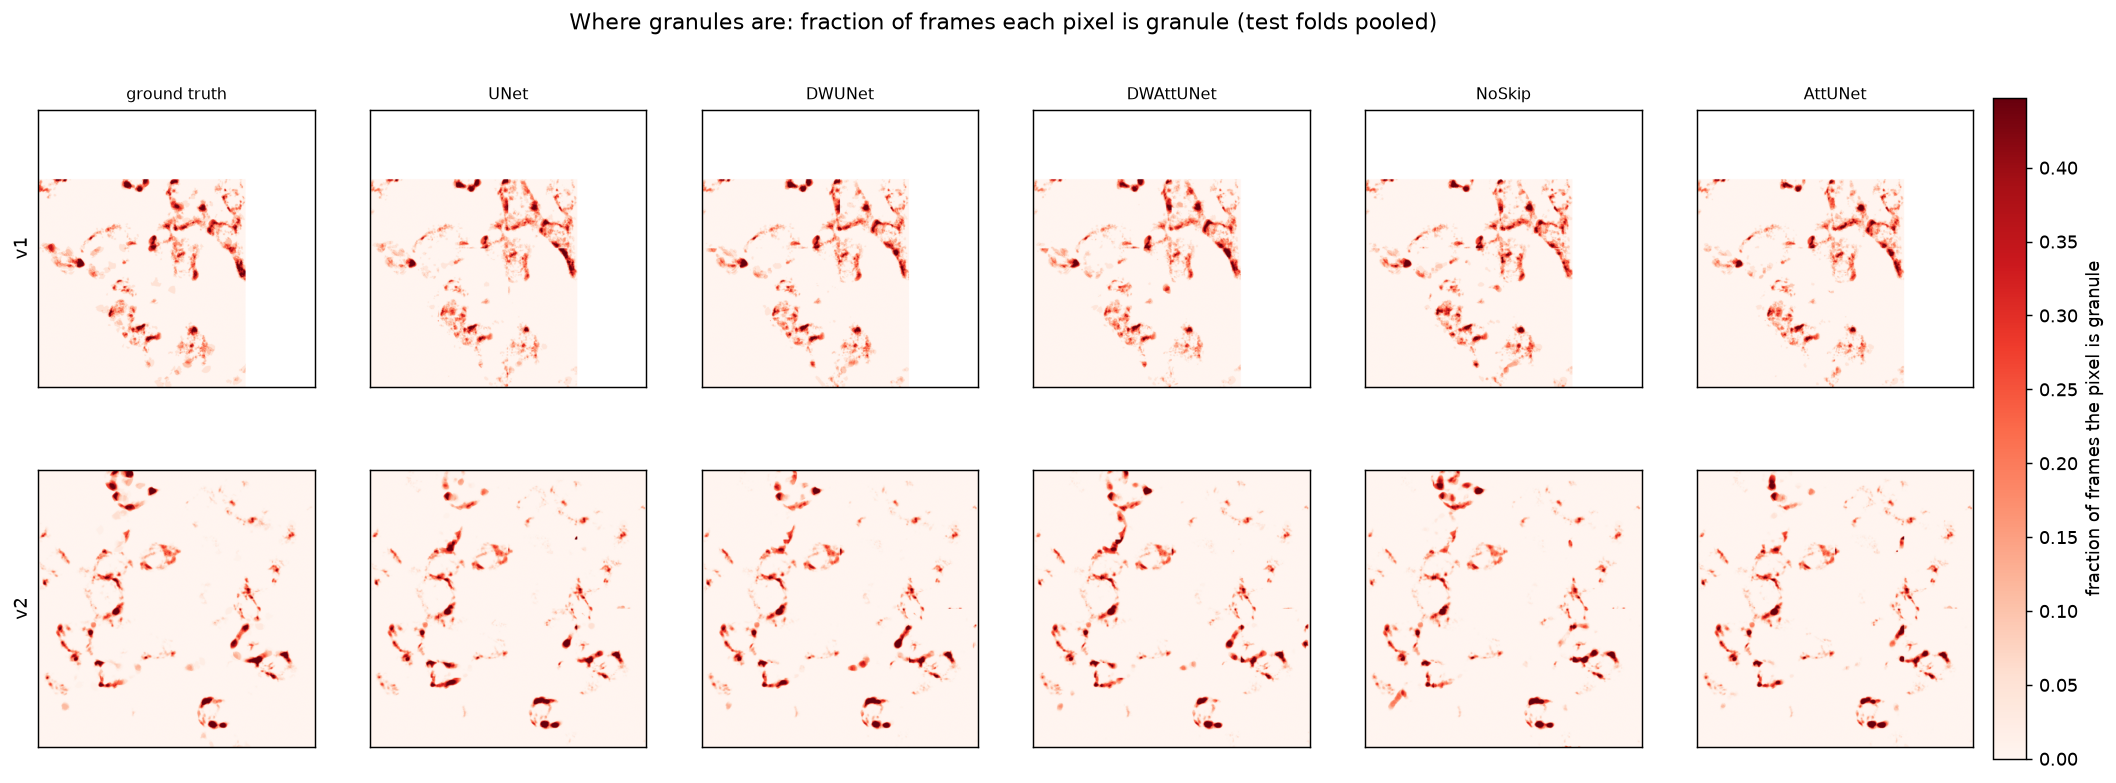
\includegraphics[width=\linewidth]{heat_occupancy.png}

  \vspace{2mm}
  \keyidea{All five networks put granules in the same places as the labels, around the same cells, in both videos:
  they learned \emph{where} granules are, not just how many. The darkest spots are granules that persist through much of the video.}
  \src{Colour = fraction of frames in which the pixel is granule; all 5-fold test sets pooled. Top: video 1, bottom: video 2.
  In video 1 the white area (top and right) has no test tile, so it is empty, not granule-free.}
\end{frame}

\begin{frame}{Backup: hand-labelled tiles 1--4, every method (red = granule)}
  \centering
  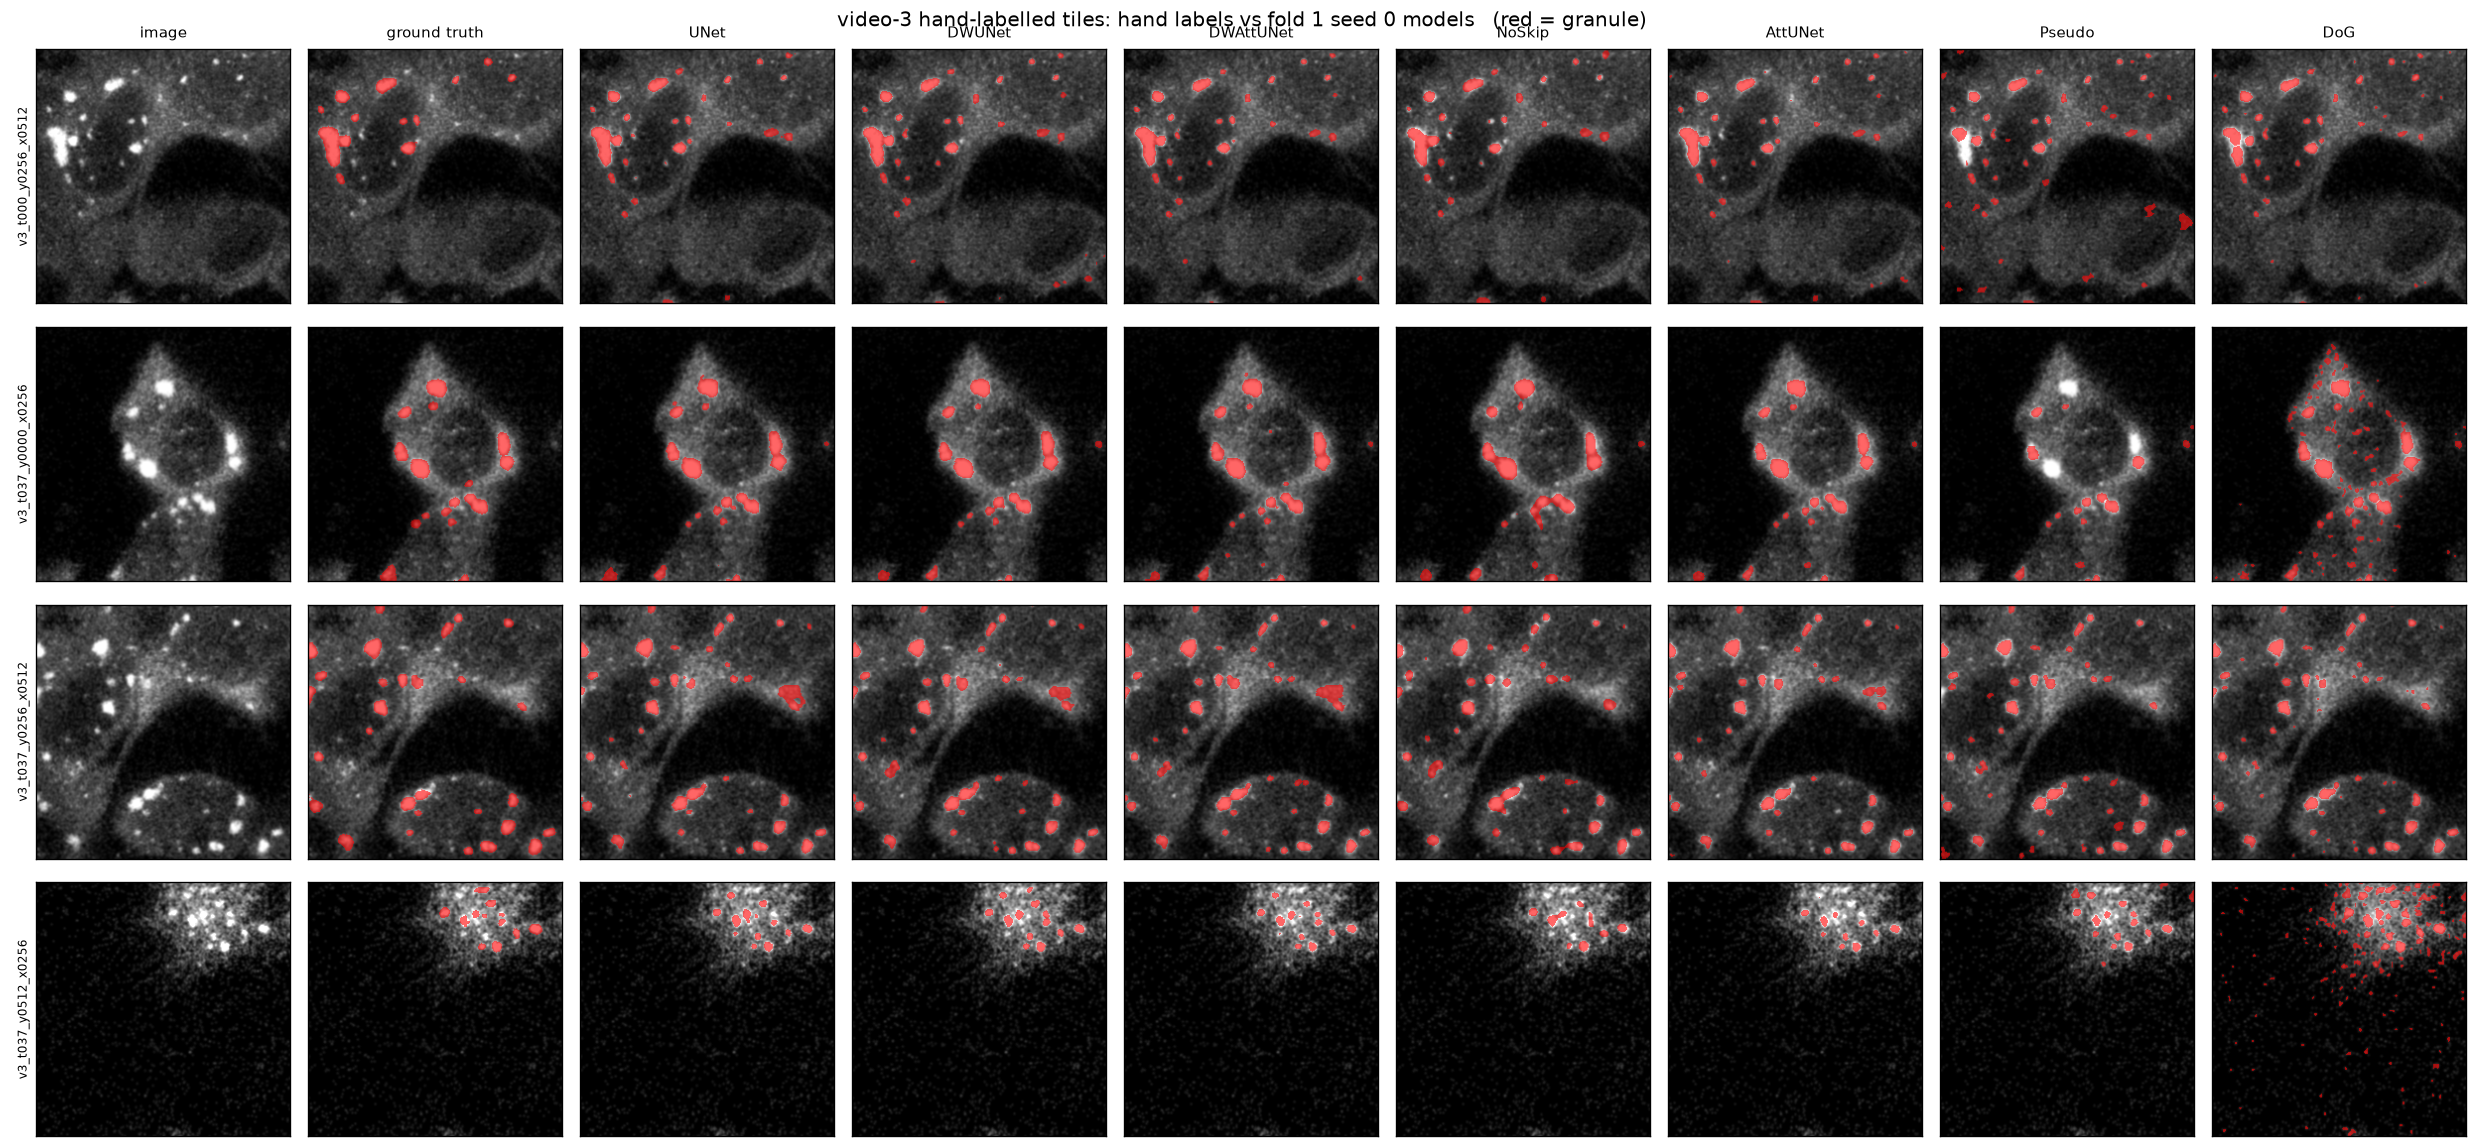
\includegraphics[height=6.1cm,keepaspectratio]{heat_hand_1.png}
  \vfill
  \src{Columns: image, hand labels, UNet, DWUNet, DWAttUNet, NoSkip, AttUNet, labeller (``Pseudo''), DoG. Fold-1 checkpoints, before the blob filter.
  Row 2: the labeller column is empty (its mask for this tile is missing, hence ``7 tiles''). Row 4: DoG sprays specks over the noisy background.}
\end{frame}

\begin{frame}{Backup: hand-labelled tiles 5--8, every method (red = granule)}
  \centering
  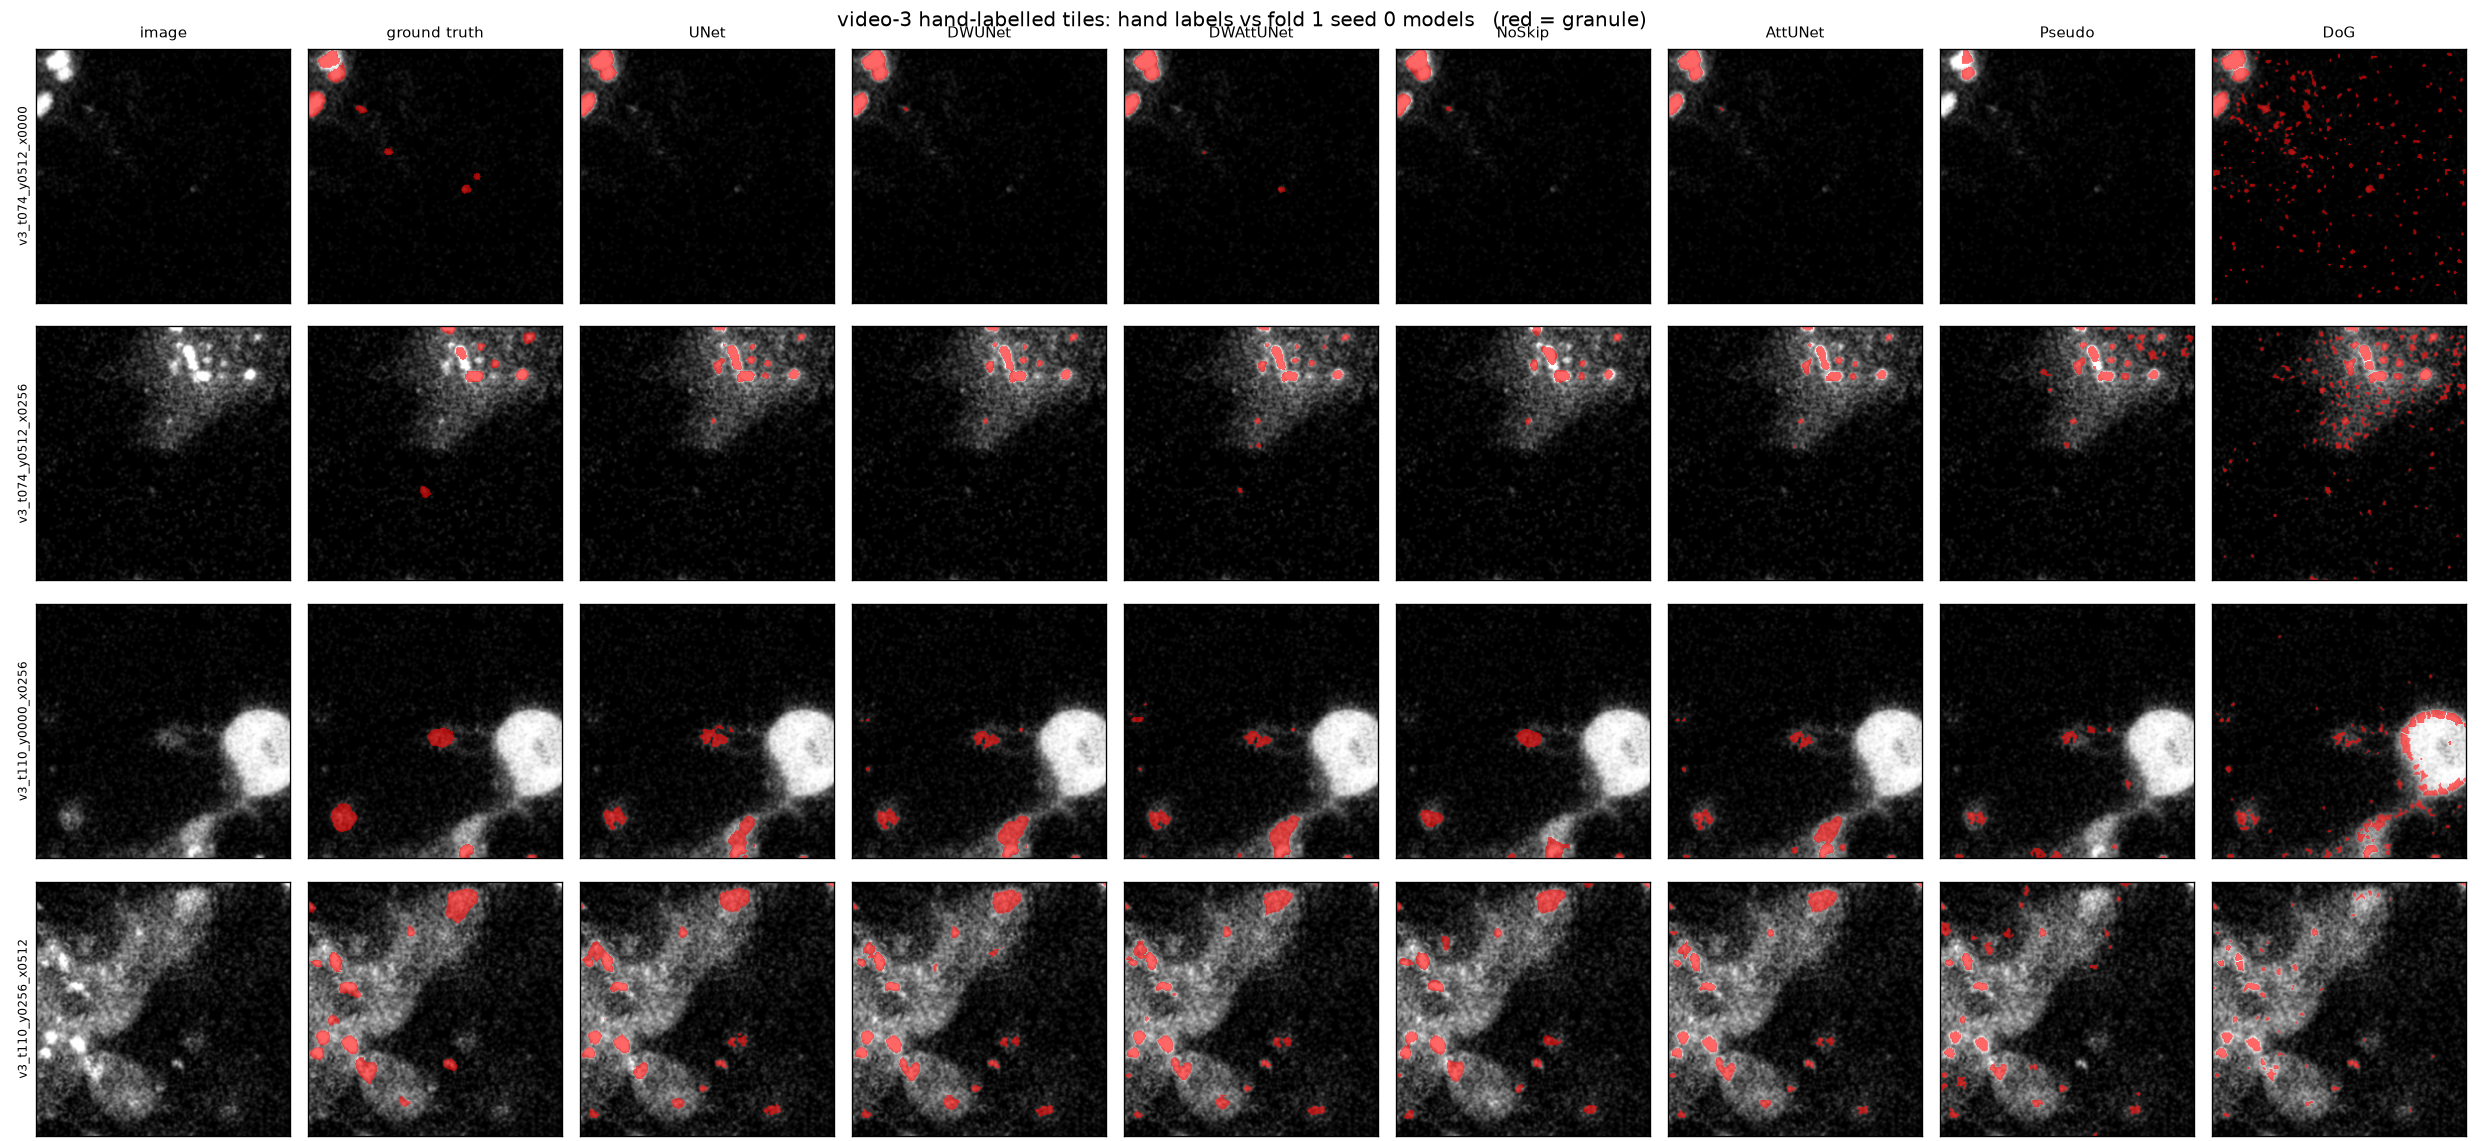
\includegraphics[height=6.1cm,keepaspectratio]{heat_hand_2.png}
  \vfill
  \src{Same columns as the previous slide. Rows 1--2: DoG floods empty background with false positives; the networks stay clean.
  Row 3: DoG outlines the bright cell body as a granule, the networks do not. Large granules match the hand outlines in every network.}
\end{frame}

\begin{frame}{Backup: a whole video-2 frame, labels vs UNet}
  \centering
  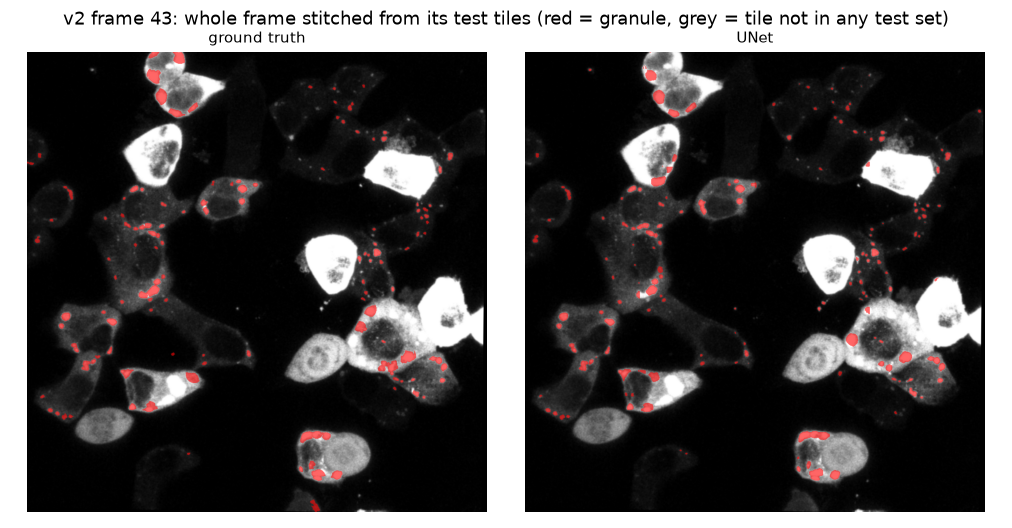
\includegraphics[height=6.0cm,keepaspectratio]{heat_frame_v2.png}
  \vfill
  \src{Video 2, frame 43, stitched from its 5-fold test tiles: every tile is predicted by the model that never saw it. Red = granule.
  The video-1 frame is on slide I.6.}
\end{frame}

\begin{frame}{Backup: 5-fold test tiles, labels vs UNet}
  \begin{columns}[c]
    \begin{column}{0.58\textwidth}\centering
      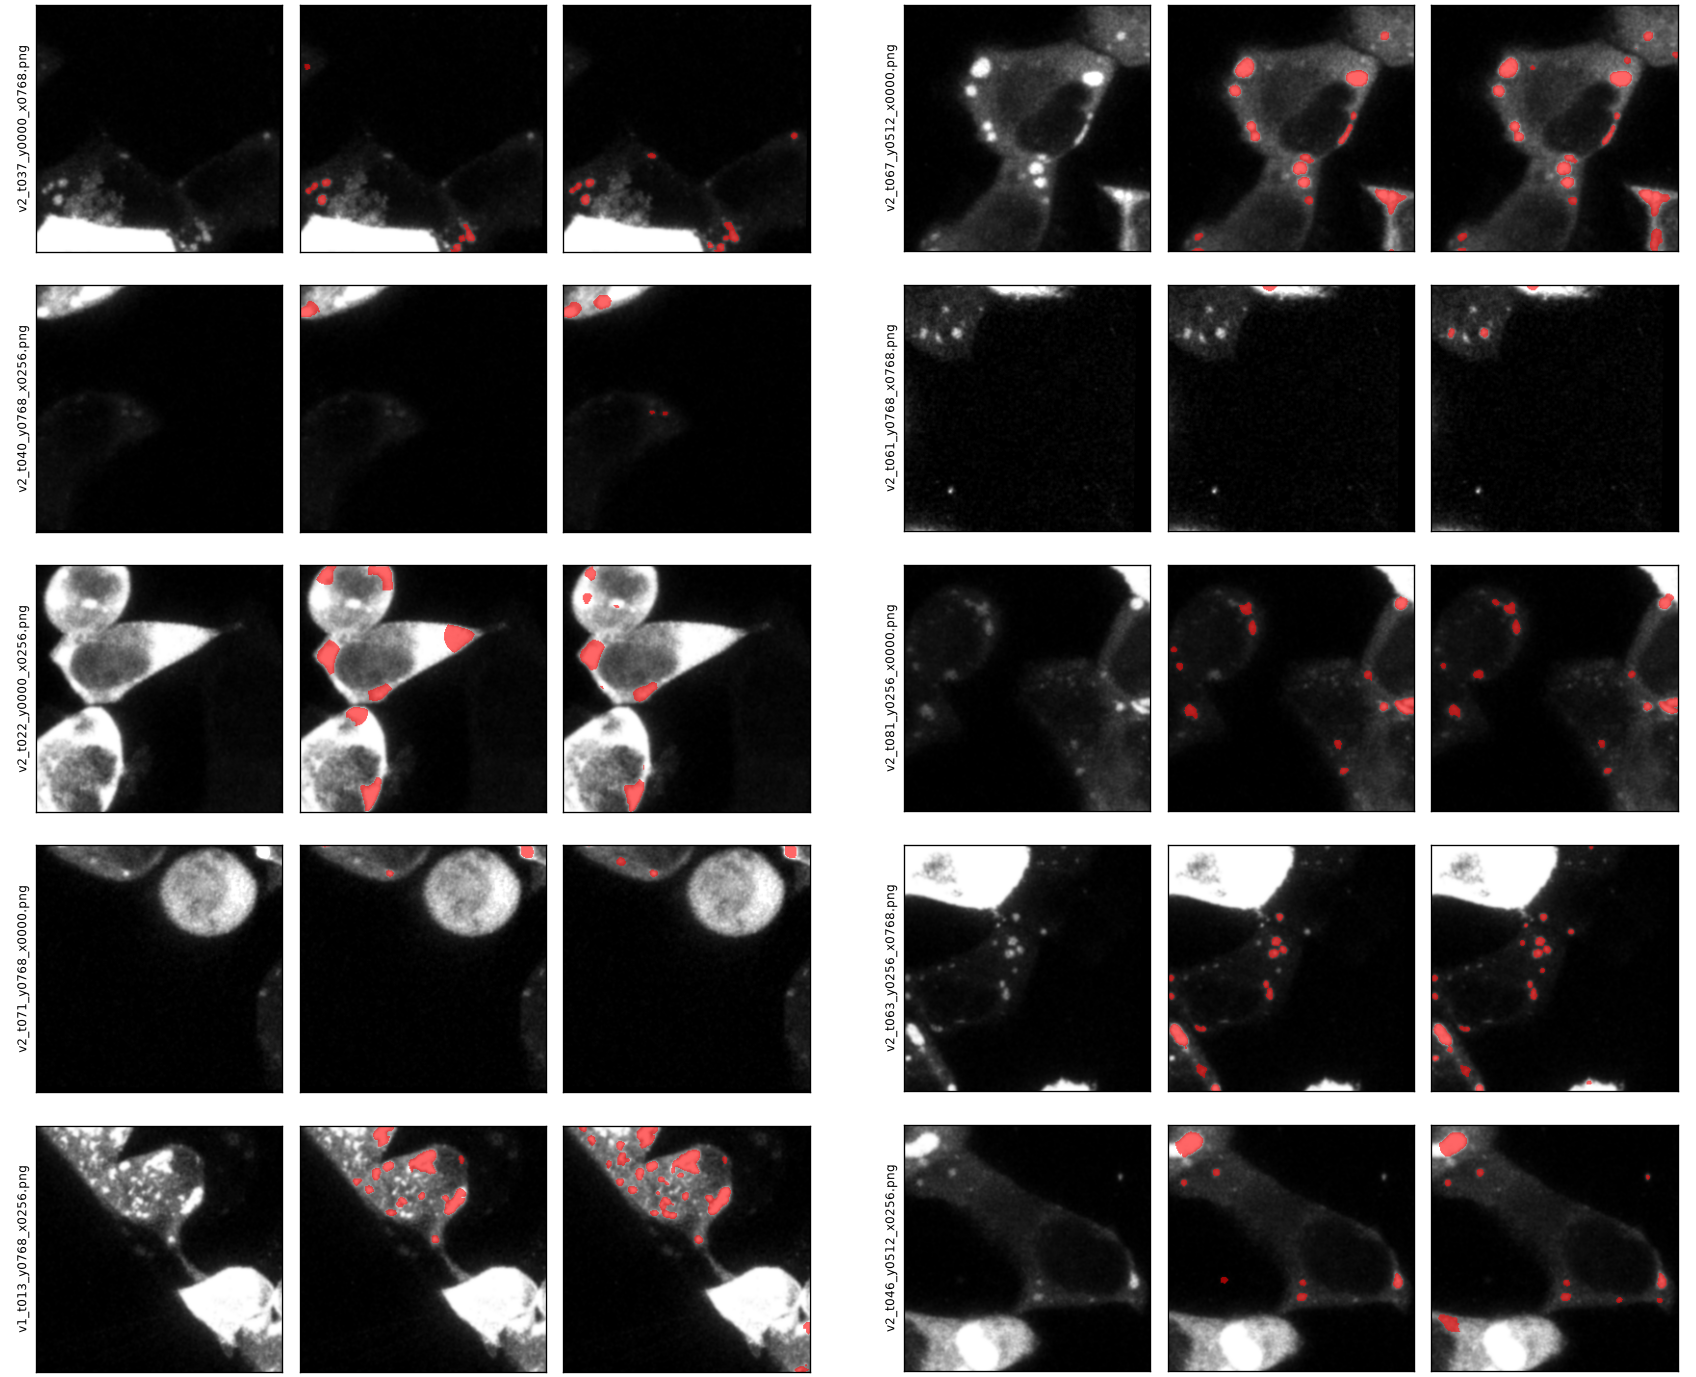
\includegraphics[height=6.4cm,keepaspectratio]{heat_folds_tiles.png}
    \end{column}
    \begin{column}{0.40\textwidth}\small
      Two test tiles per fold. In each group of three: \textbf{image}, \textbf{labels} (V4 pseudo-labels), \textbf{UNet}.\par\vspace{3mm}
      UNet reproduces the labelled granules closely, including the large ones, and adds a few small extra blobs ---
      the blobs the 20 px filter removes.\par\vspace{3mm}
      {\color{muted}\footnotesize Before the blob filter; red = granule.}
    \end{column}
  \end{columns}
\end{frame}

\end{document}
